\documentclass{article}
\usepackage{graphicx} % Required for inserting images
\usepackage{minted} % Required for colored code and image rendering
\usepackage[a4paper, left=1.5in, right=1in, top=.5in, bottom=.5in]{geometry} % Page layout
\begin{document}
\section{EXPERIMENT 1} % experiment heading goes here
\textbf{Aim}
\begin{flushleft}
% replace with relevant experiment's aim
Explore the usage of following commands. For each of the command, write an illustrative
example along with its output.
\end{flushleft}
% use the below code to typeset code or any similar content from the aim in monospace font
\begin{verbatim}
ps, pstree, strace, gdb, strings, objdump, nm, file, od, xxd, fuser, top, awk,
cal, ls, chmod, chown, chgrp, mkdir, rmdir, locate, nftw, touch, cat, more,
less, cp, mv, rm, grep, tail, head, find, sort, stty, sed, uniq, du, df, man,
help, pr, tr, diff, wc, bc, gzip, history, groups, cut
\end{verbatim}
\subsection{Command 1: ps} 
\textbf{Purpose}
\begin{flushleft}
 process status
\end{flushleft}
\textbf{Usage}
\begin{verbatim}
ps
ps axjf
ps axms
\end{verbatim}
\textbf{Sample i/p and o/p}
\begin{figure}[H] 
\fbox{
\begin{minipage}{350px} 
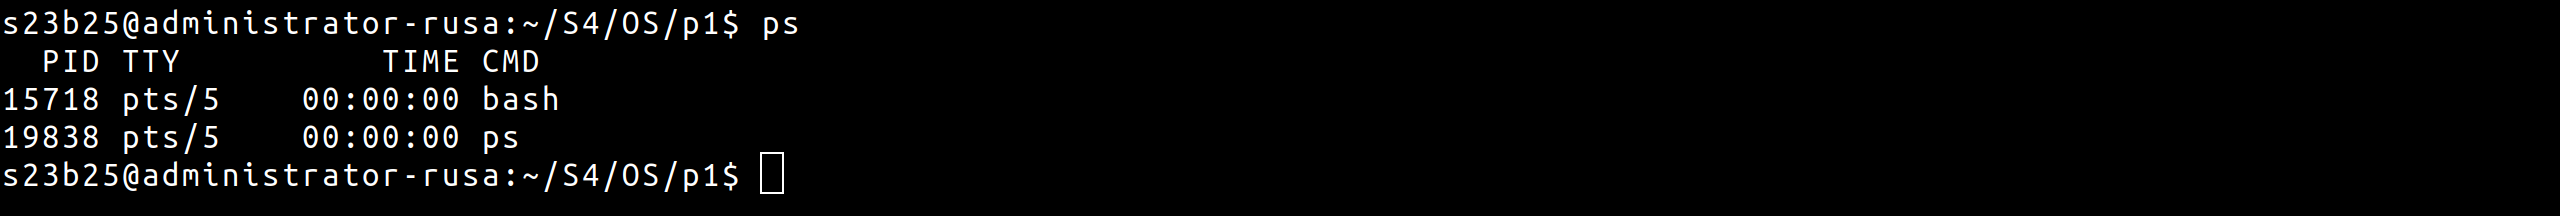
\includegraphics[width=\linewidth]{assets/ps-1.png}
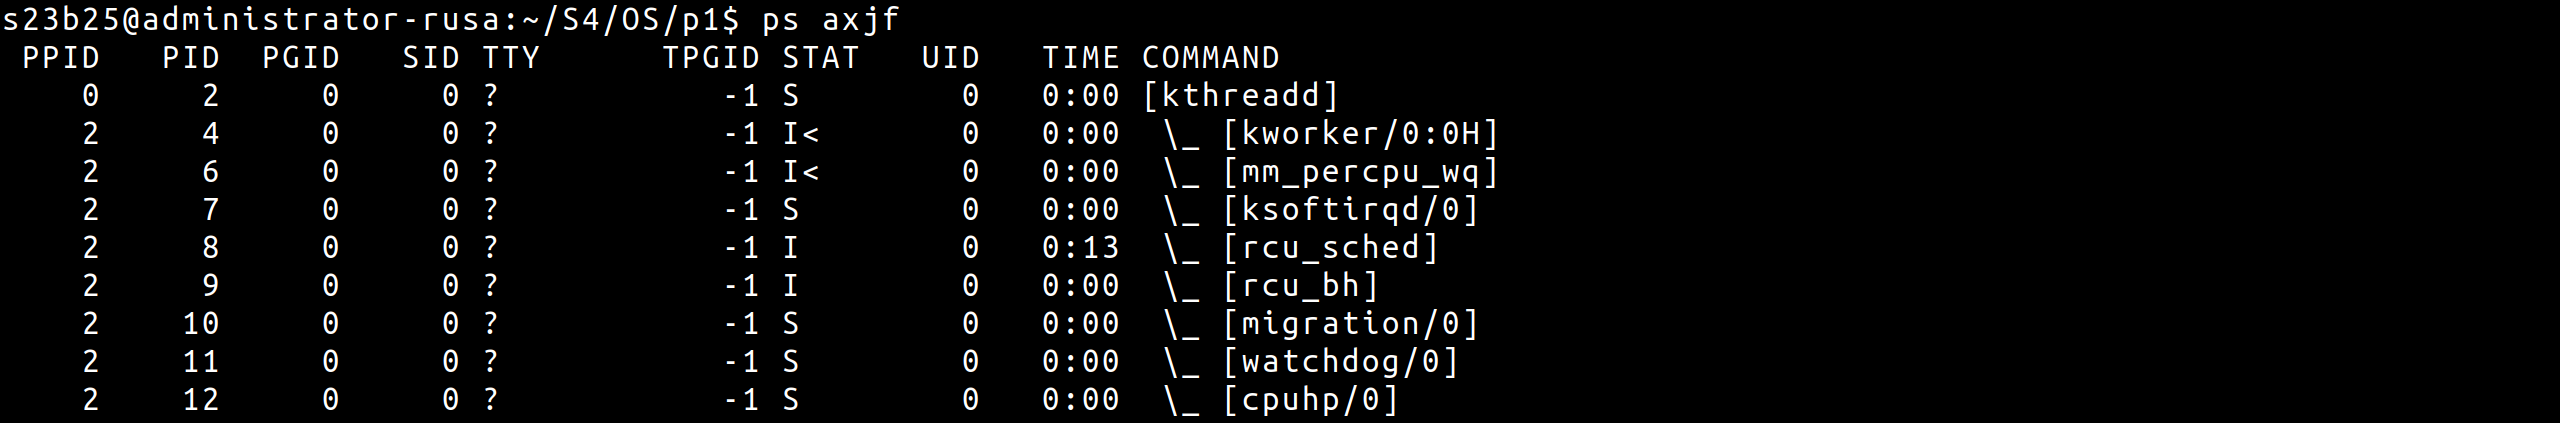
\includegraphics[width=\linewidth]{assets/ps-2.png}
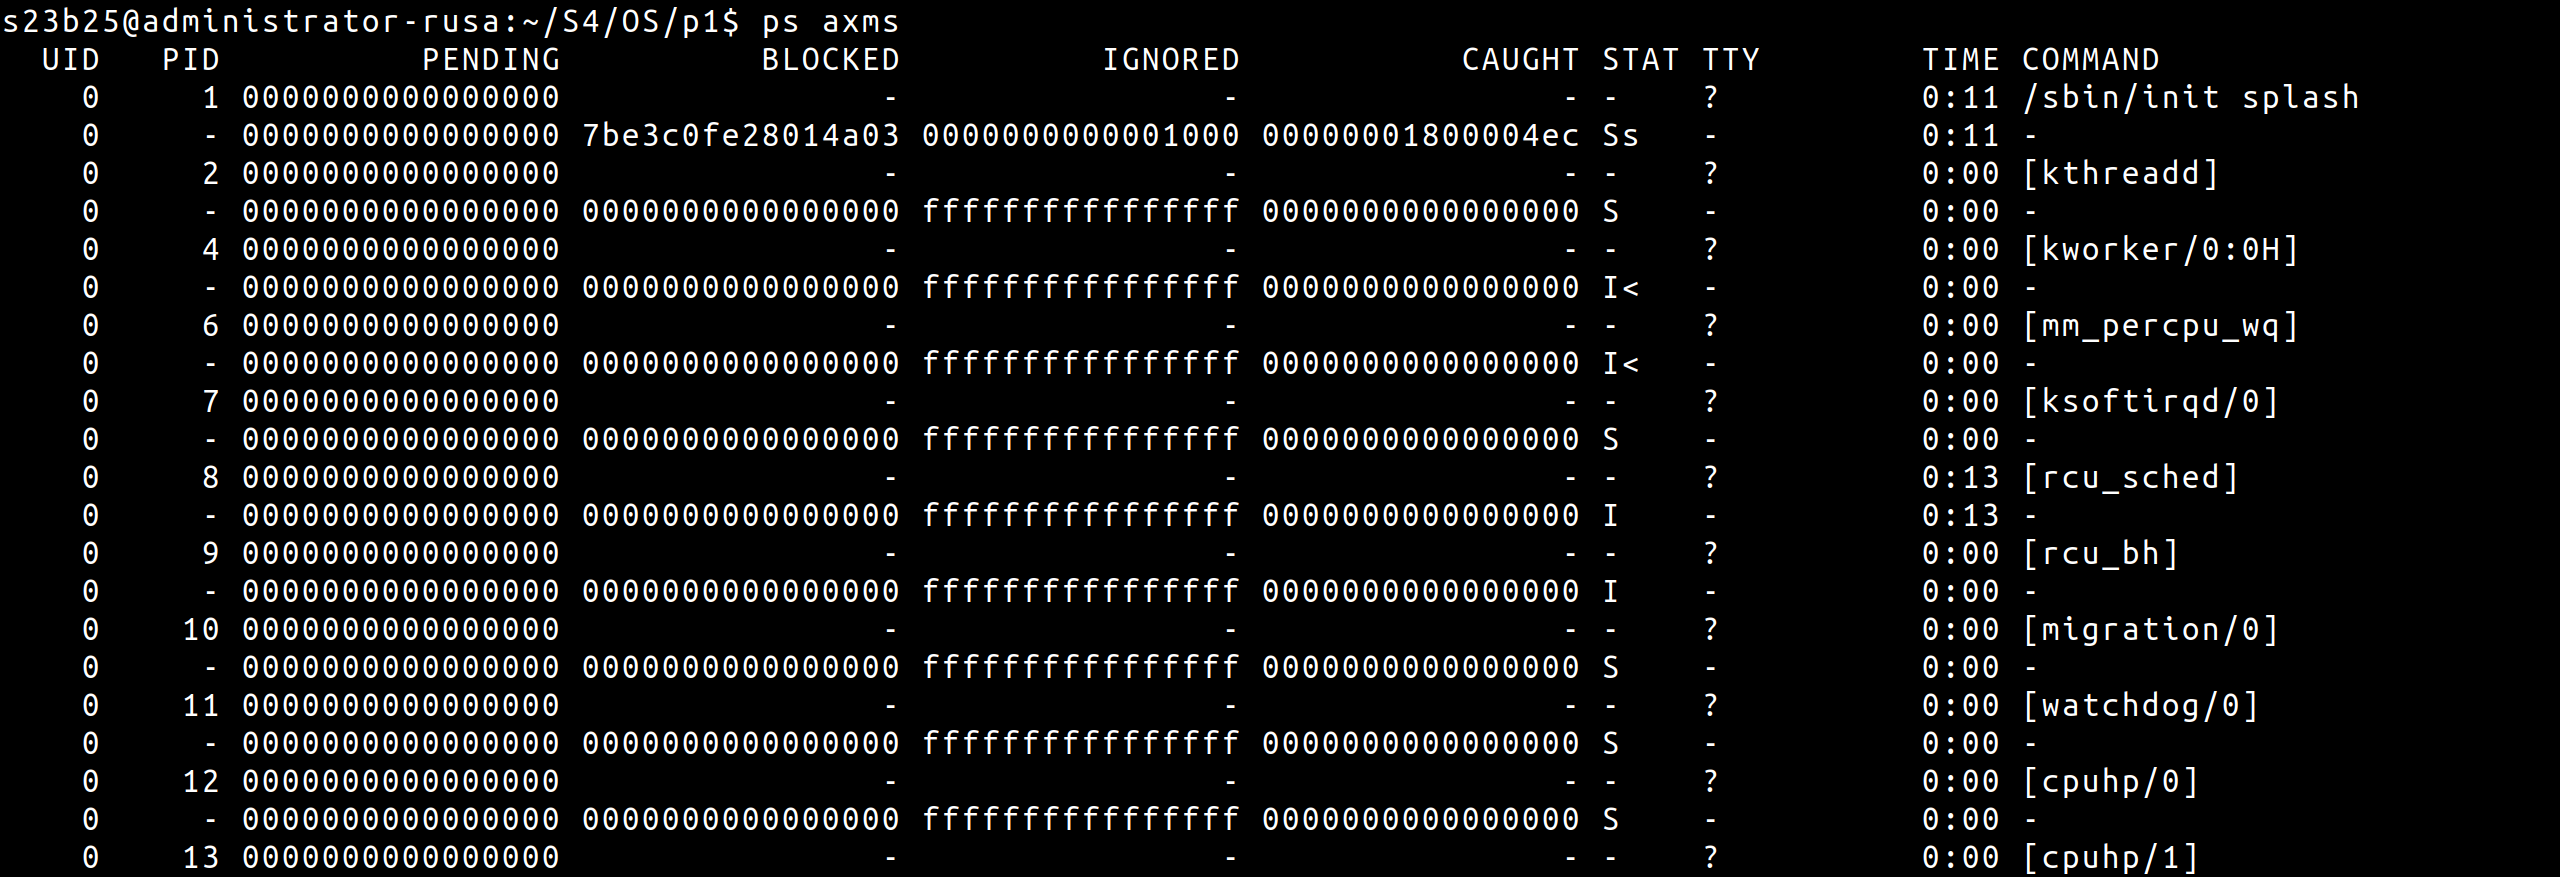
\includegraphics[width=\linewidth]{assets/ps-3.png}
\end{minipage}
} %output screenshot name
\end{figure}
\subsection{Command 2: pstree} 
\textbf{Purpose}
\begin{flushleft}
display a tree of processes
\end{flushleft}
\textbf{Usage}
\begin{verbatim}
pstree
pstree -c
pstree -p
\end{verbatim}
\textbf{Sample i/p and o/p}
\begin{figure}[H] 
\fbox{
\begin{minipage}{350px} 
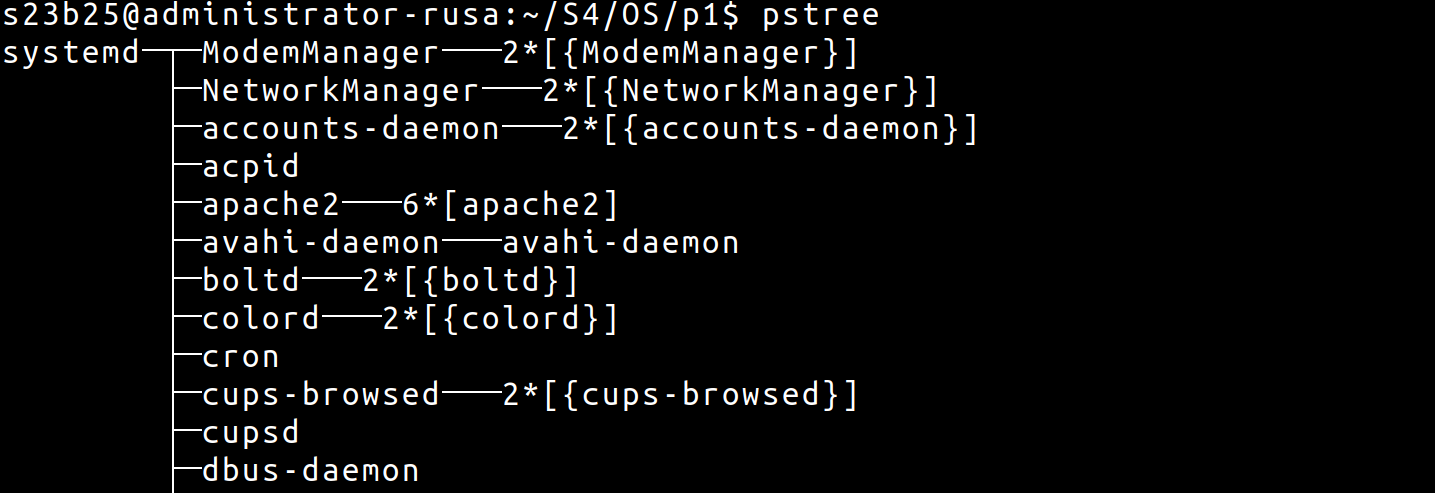
\includegraphics[width=\linewidth]{assets/pstree-1.png}
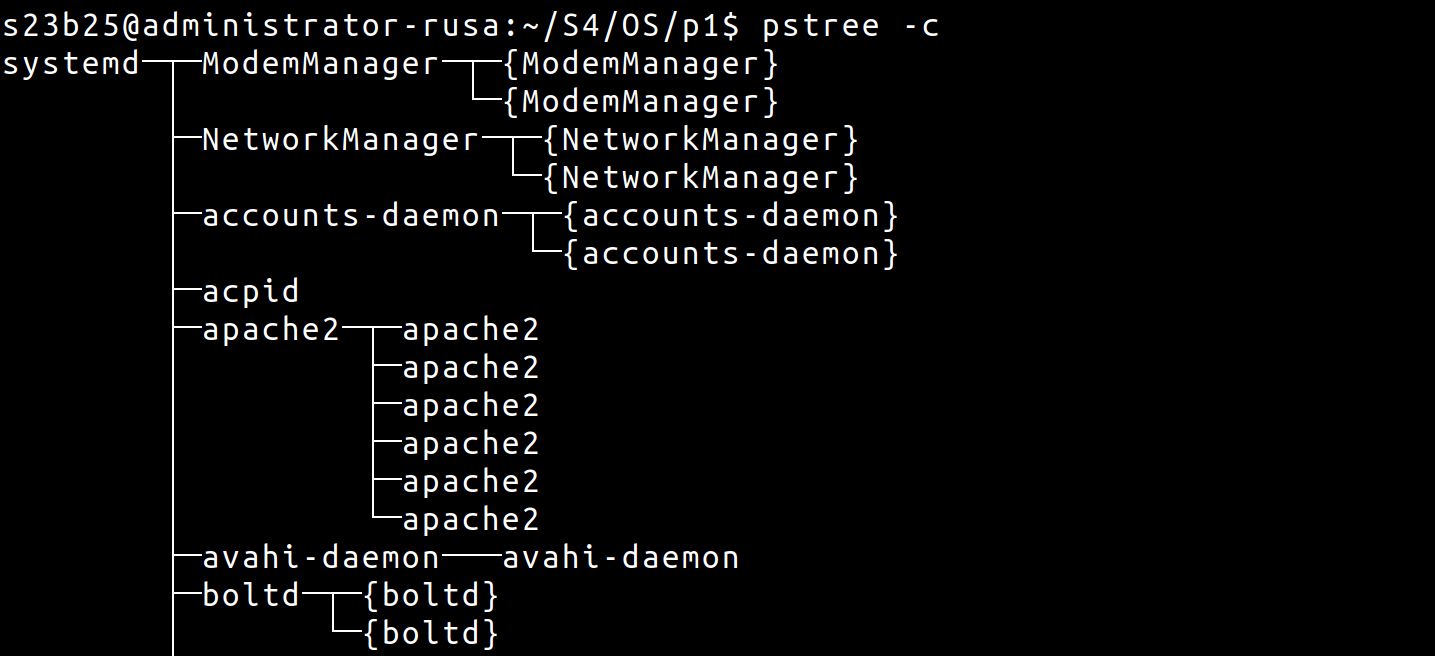
\includegraphics[width=\linewidth]{assets/pstree-2.png}
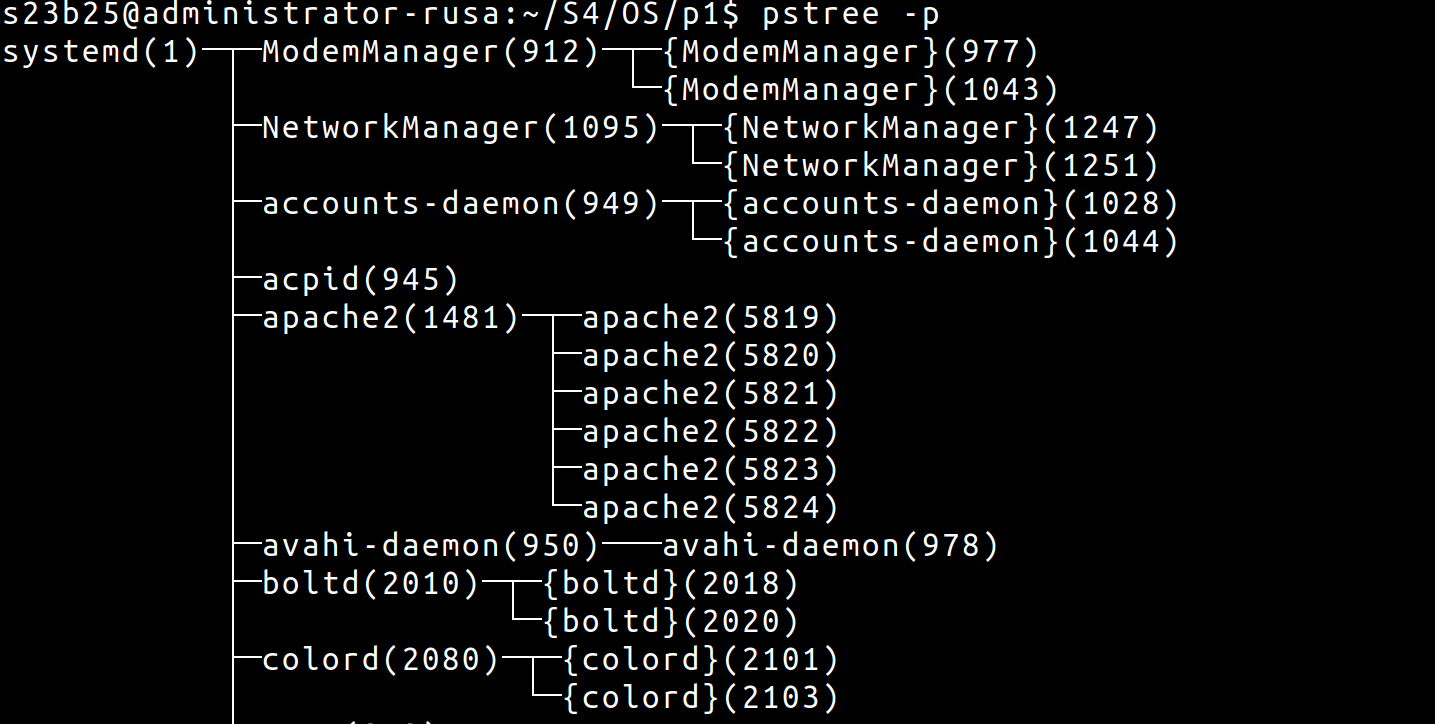
\includegraphics[width=\linewidth]{assets/pstree-3.png}
\end{minipage}
} %output screenshot name
\end{figure}
\subsection{Command 3: strace} 
\textbf{Purpose}
\begin{flushleft}
trace system calls and signals
\end{flushleft}
\textbf{Usage}
\begin{verbatim}
strace gedit
\end{verbatim}
\textbf{Sample i/p and o/p}
\begin{figure}[H] 
\fbox{
\begin{minipage}{350px} 
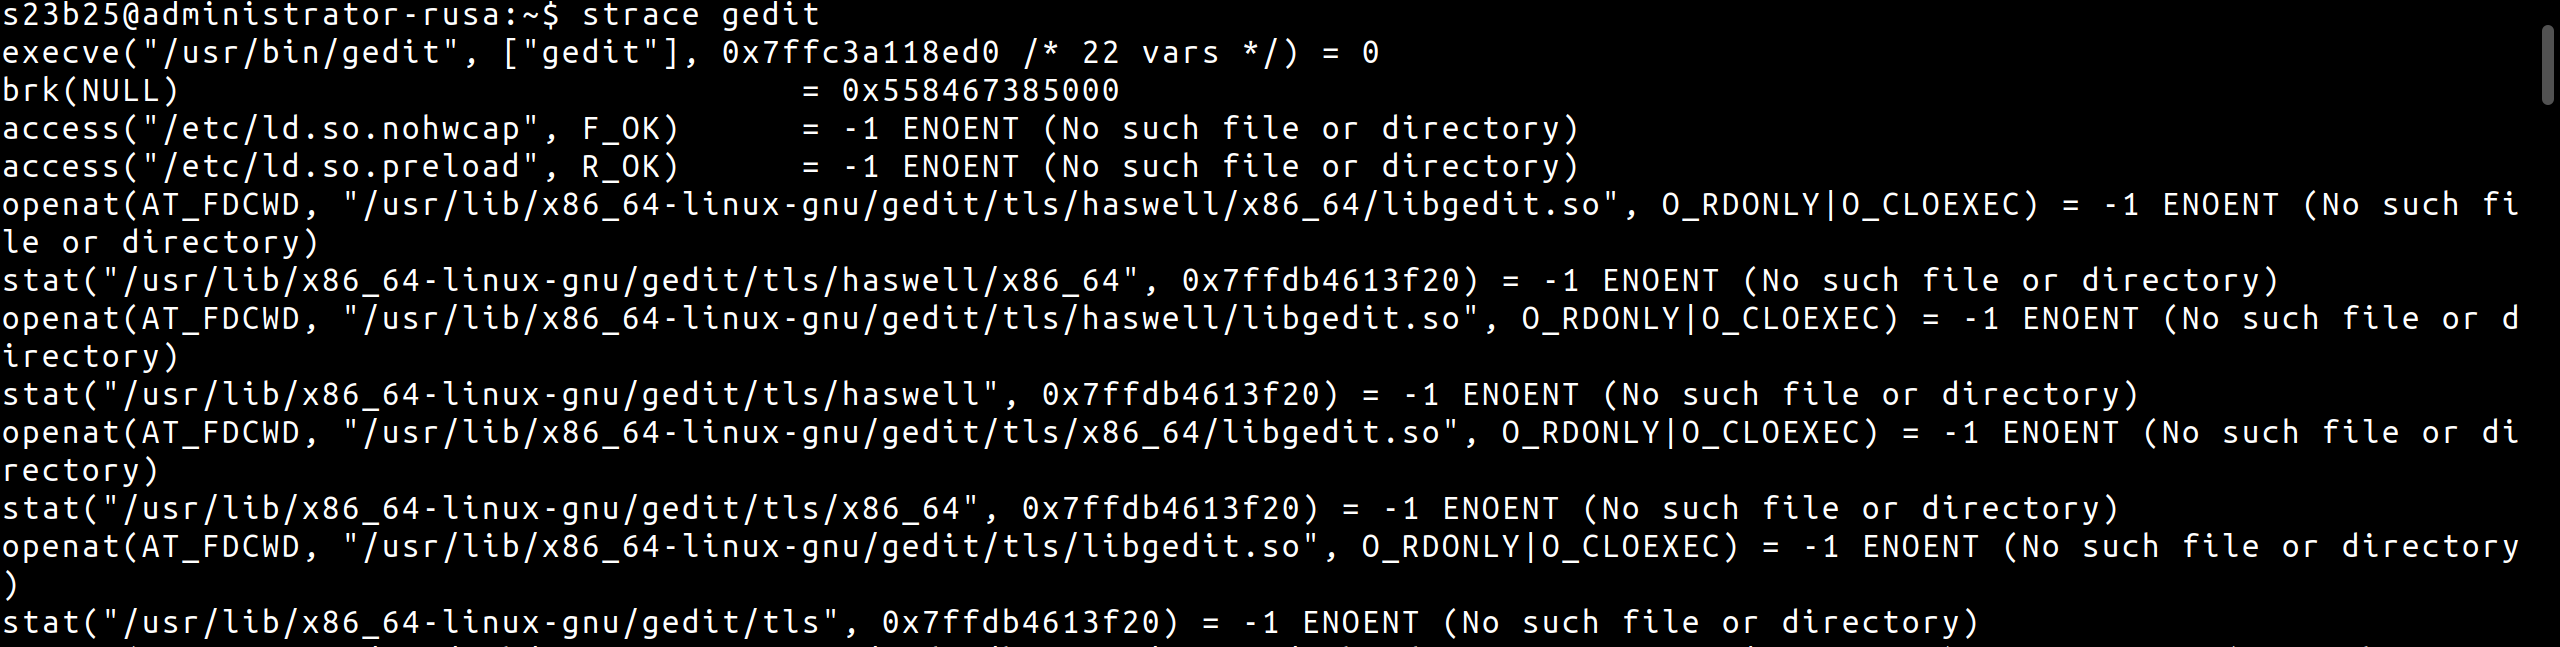
\includegraphics[width=\linewidth]{assets/strace-1.png}
\end{minipage}
} %output screenshot name
\end{figure}
\subsection{Command 4: gdb} 
\textbf{Purpose}
\begin{flushleft}
the GNU Debugger
\end{flushleft}
\textbf{Usage}
\begin{verbatim}
gdb ./a.out
\end{verbatim}
\textbf{Sample i/p and o/p}
\begin{figure}[H] 
\fbox{
\begin{minipage}{350px} 
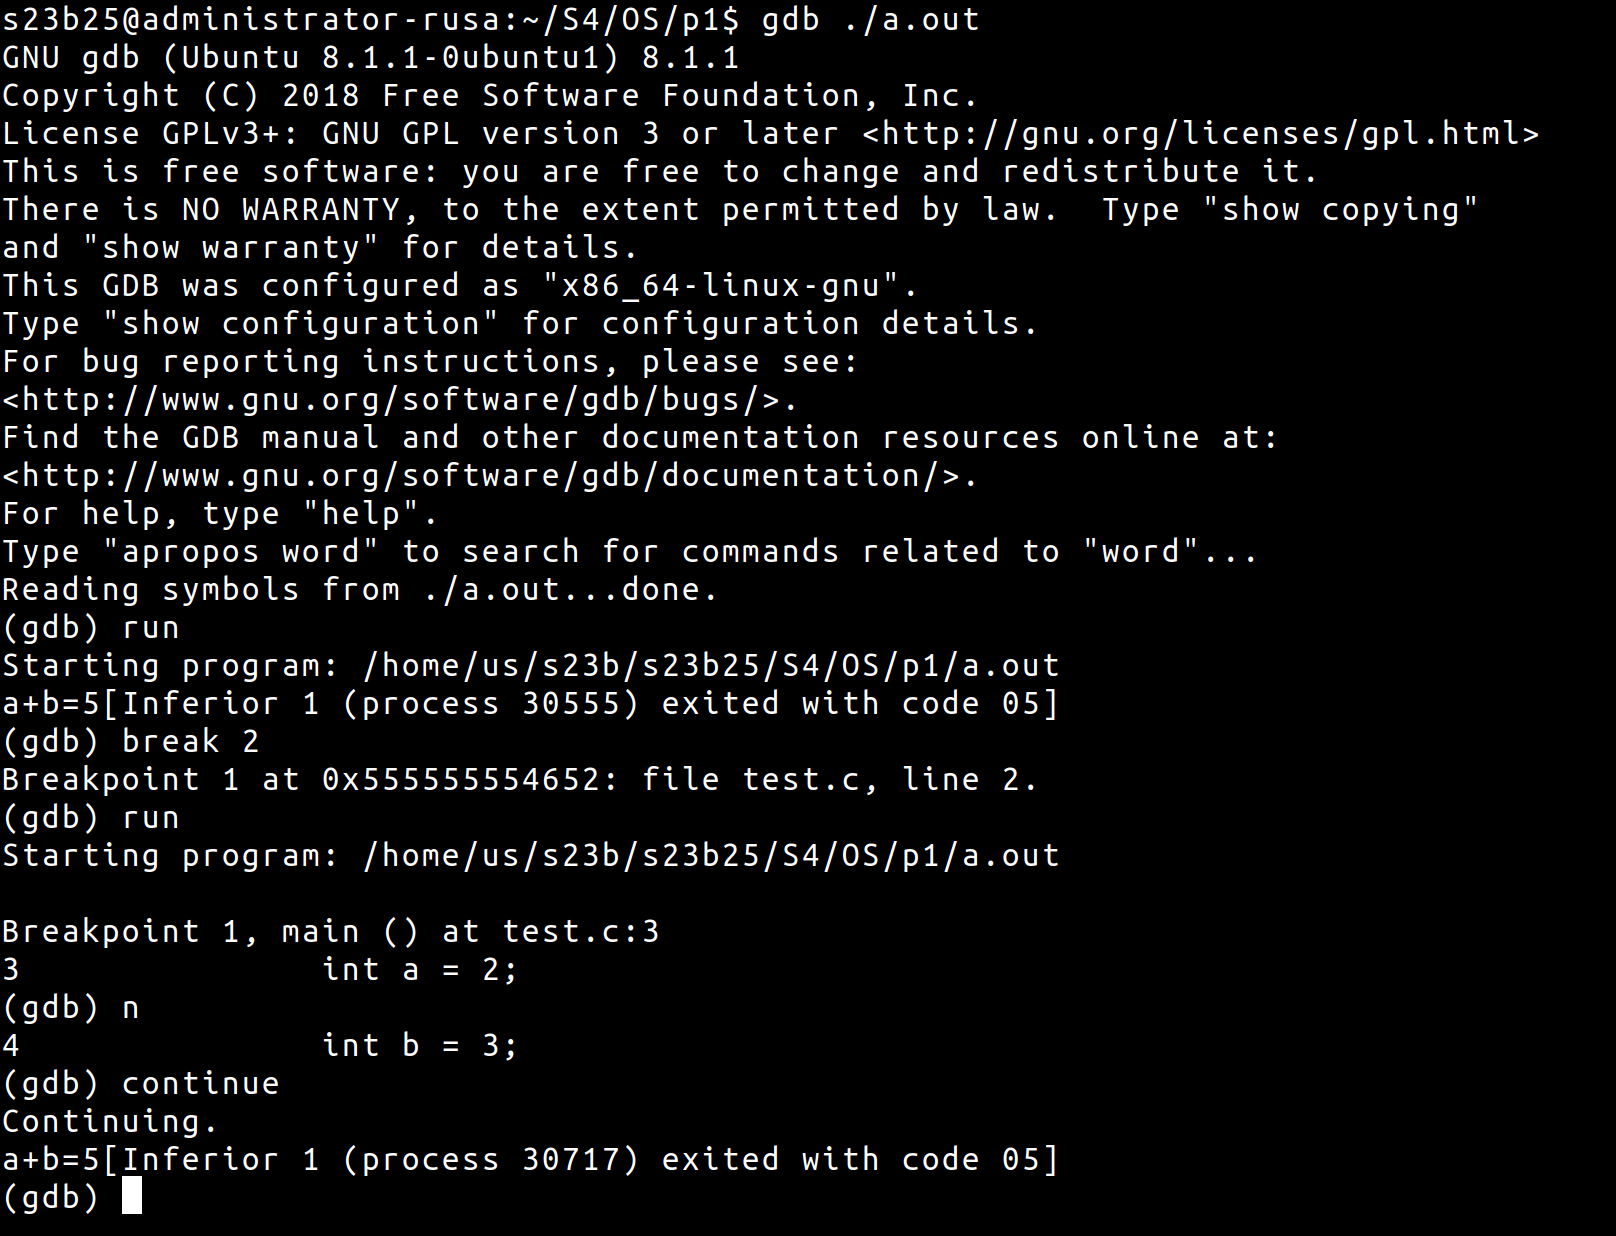
\includegraphics[width=\linewidth]{assets/gdb-1.png}
\end{minipage}
} %output screenshot name
\end{figure}
\subsection{Command 5: strings} 
\textbf{Purpose}
\begin{flushleft}
       strings - find the printable strings in a object, or other binary, file
\end{flushleft}
\textbf{Usage}
\begin{verbatim}
strings test.c
\end{verbatim}
\textbf{Sample i/p and o/p}
\begin{figure}[H] 
\fbox{
\begin{minipage}{350px} 
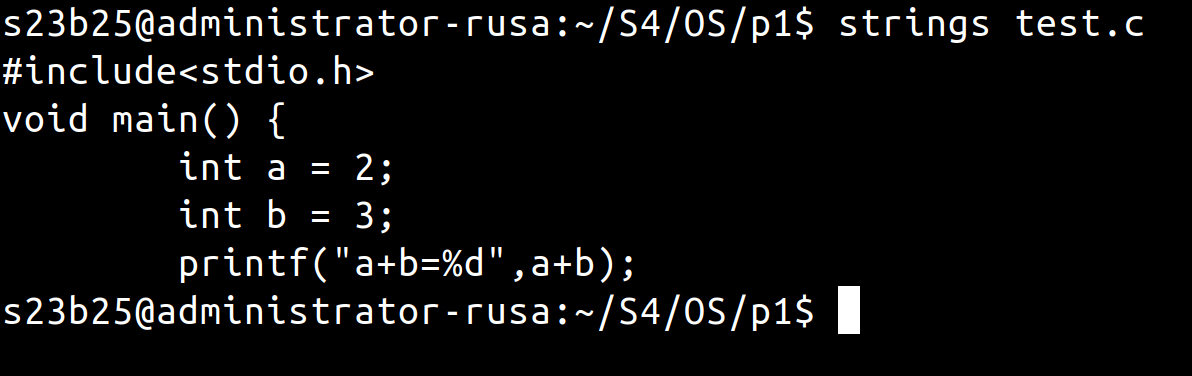
\includegraphics[width=\linewidth]{assets/strings-1.png}
\end{minipage}
} %output screenshot name
\end{figure}
\subsection{Command 6: objdump} 
\textbf{Purpose}
\begin{flushleft}
       llvm-objdump - LLVM's object file dumper
\end{flushleft}
\textbf{Usage}
\begin{verbatim}
objdump -f ./a.out
objdump -S ./a.out
\end{verbatim}
\textbf{Sample i/p and o/p}
\begin{figure}[H] 
\fbox{
\begin{minipage}{350px} 
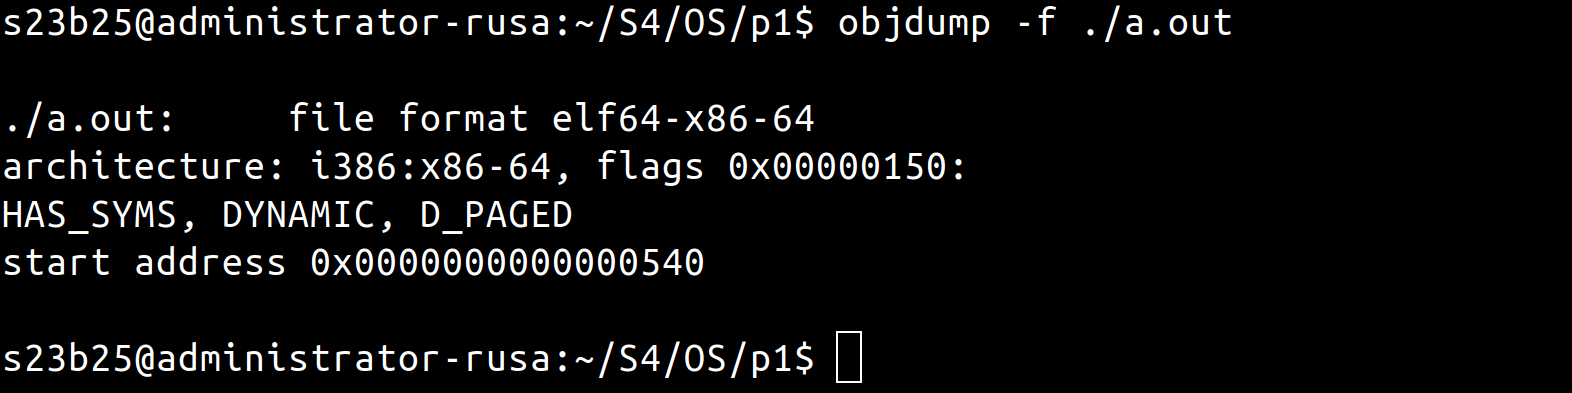
\includegraphics[width=\linewidth]{assets/objdump-2.png}
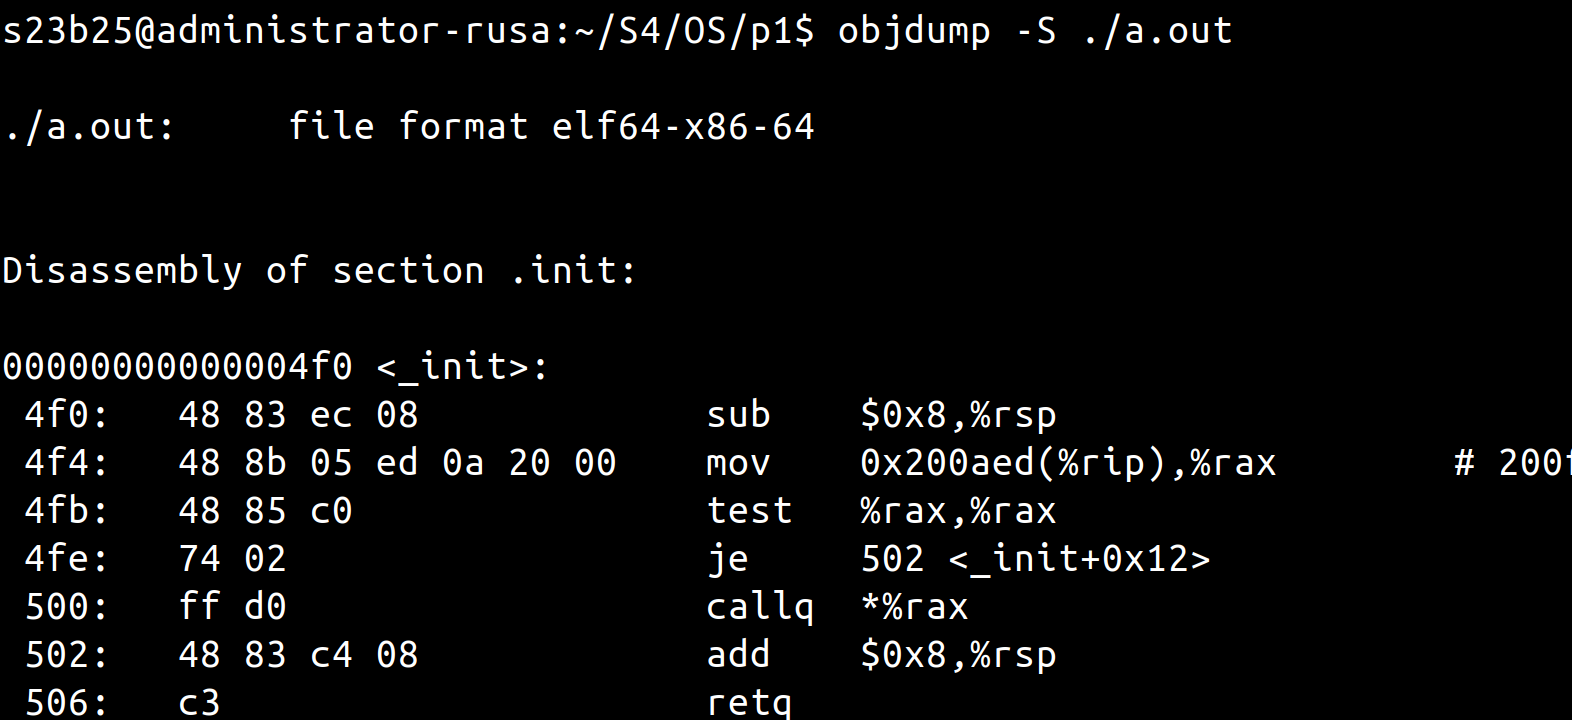
\includegraphics[width=\linewidth]{assets/objdump-3.png}
\end{minipage}
} %output screenshot name
\end{figure}
\subsection{Command 7: nm} 
\textbf{Purpose}
\begin{flushleft}
       nm - display name list (symbol table)
\end{flushleft}
\textbf{Usage}
\begin{verbatim}
nm -g
\end{verbatim}
\textbf{Sample i/p and o/p}
\begin{figure}[H] 
\fbox{
\begin{minipage}{350px} 
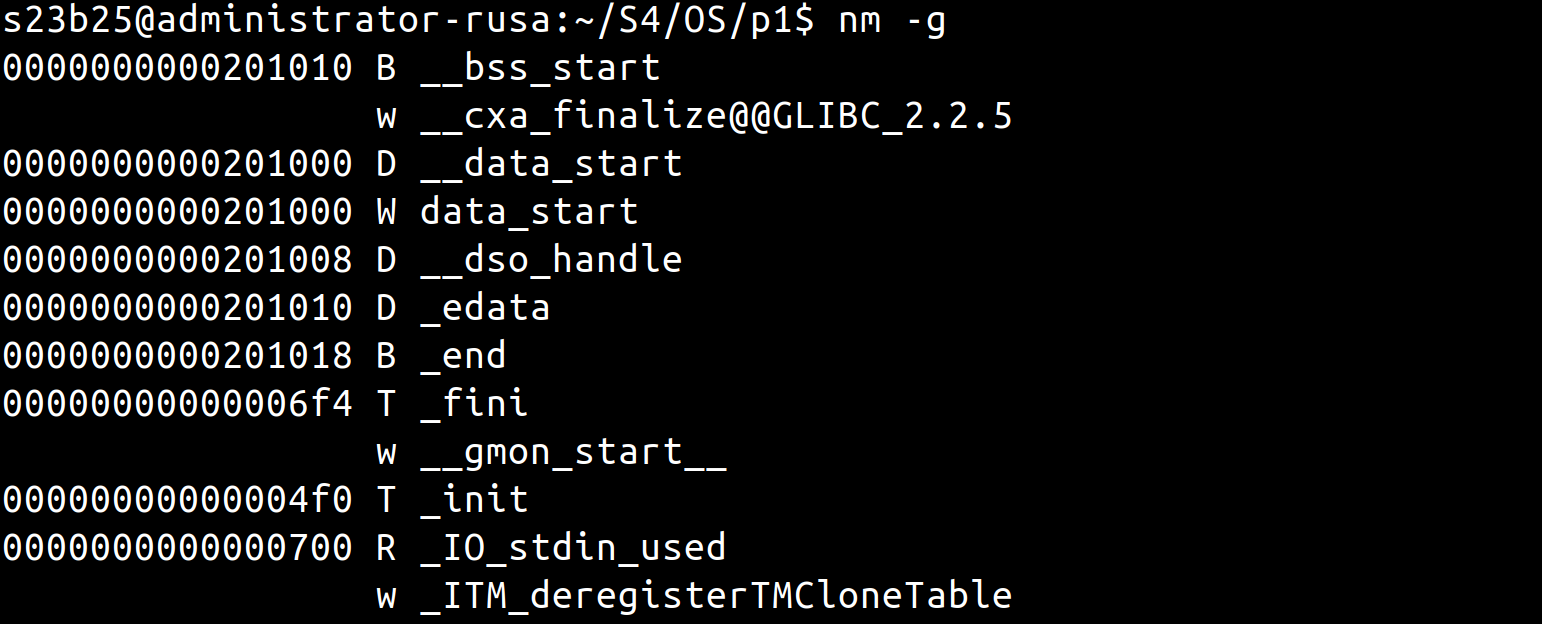
\includegraphics[width=\linewidth]{assets/nm-3.png}
\end{minipage}
} %output screenshot name
\end{figure}
\subsection{Command 8: file} 
\textbf{Purpose}
\begin{flushleft}
 determine file type
\end{flushleft}
\textbf{Usage}
\begin{verbatim}
file test.c
file --extensions test.c
file --mime-encoding test.c
\end{verbatim}
\textbf{Sample i/p and o/p}
\begin{figure}[H] 
\fbox{
\begin{minipage}{350px} 
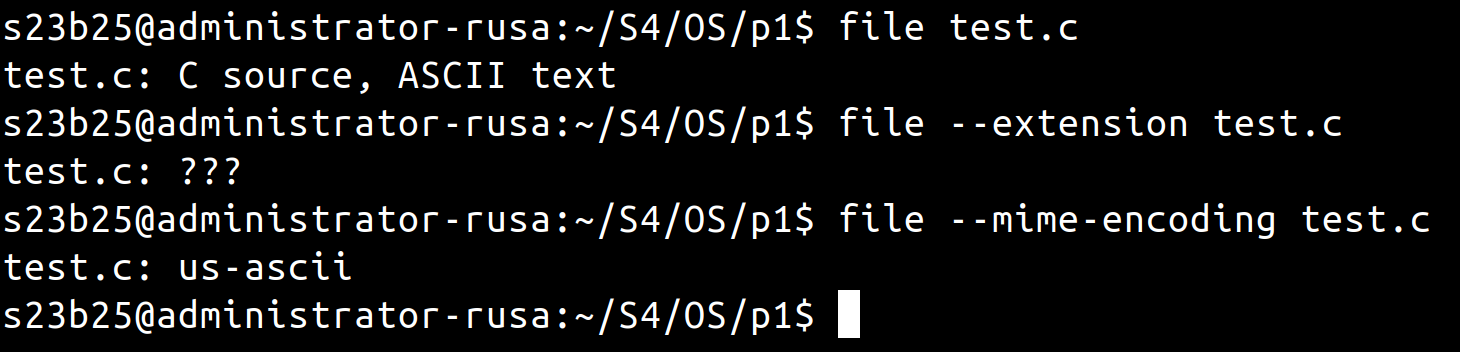
\includegraphics[width=\linewidth]{assets/file-1.png}
\end{minipage}
} %output screenshot name
\end{figure}
\subsection{Command 9: od} 
\textbf{Purpose}
\begin{flushleft}
 octal, decimal, hex, ASCII dump
\end{flushleft}
\textbf{Usage}
\begin{verbatim}
od test.c
od -a test.c
od -o test.c
\end{verbatim}
\textbf{Sample i/p and o/p}
\begin{figure}[H] 
\fbox{
\begin{minipage}{350px} 
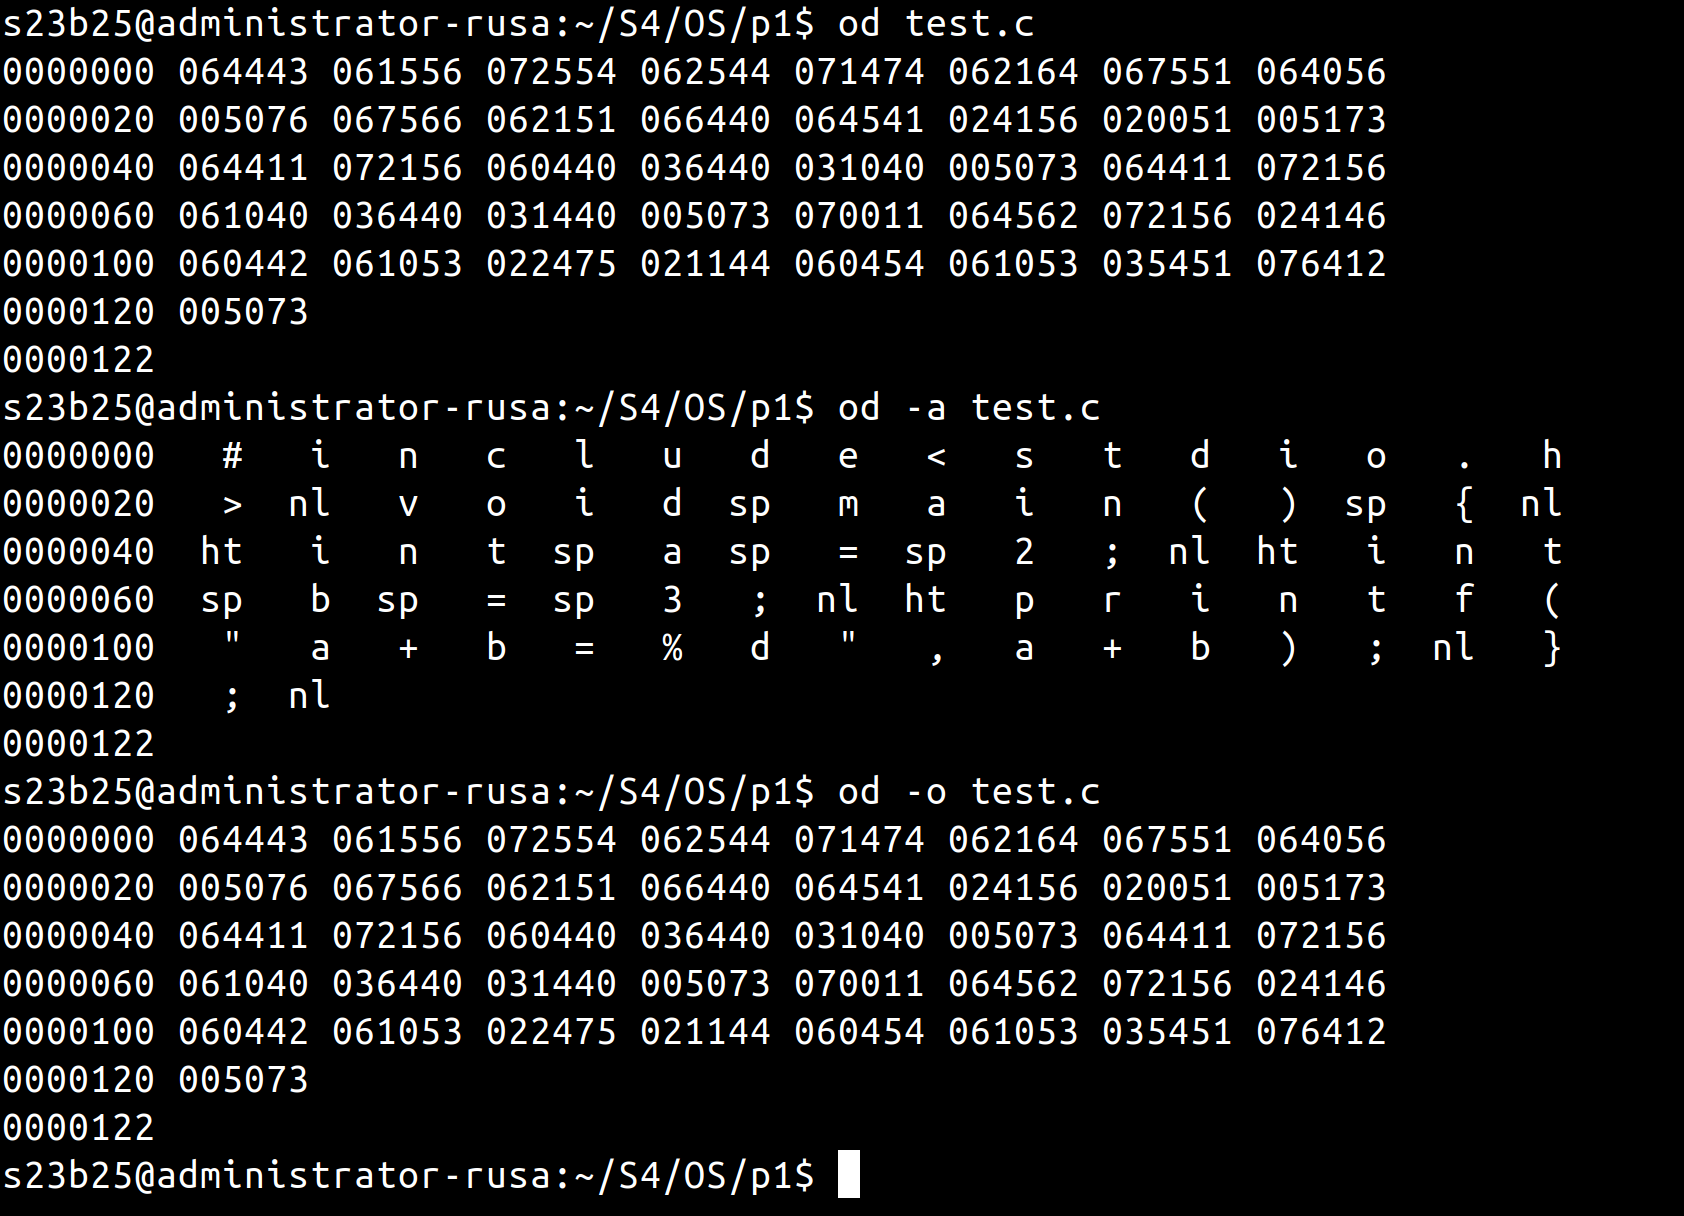
\includegraphics[width=\linewidth]{assets/od-1.png}
\end{minipage}
} %output screenshot name
\end{figure}
\subsection{Command 10: xxd} 
\textbf{Purpose}
\begin{flushleft}
       _x_x_d - make a hex dump or do the reverse.
\end{flushleft}
\textbf{Usage}
\begin{verbatim}
xxd test.c
xxd -i test.c
xxd -e test.c
\end{verbatim}
\textbf{Sample i/p and o/p}
\begin{figure}[H] 
\fbox{
\begin{minipage}{350px} 
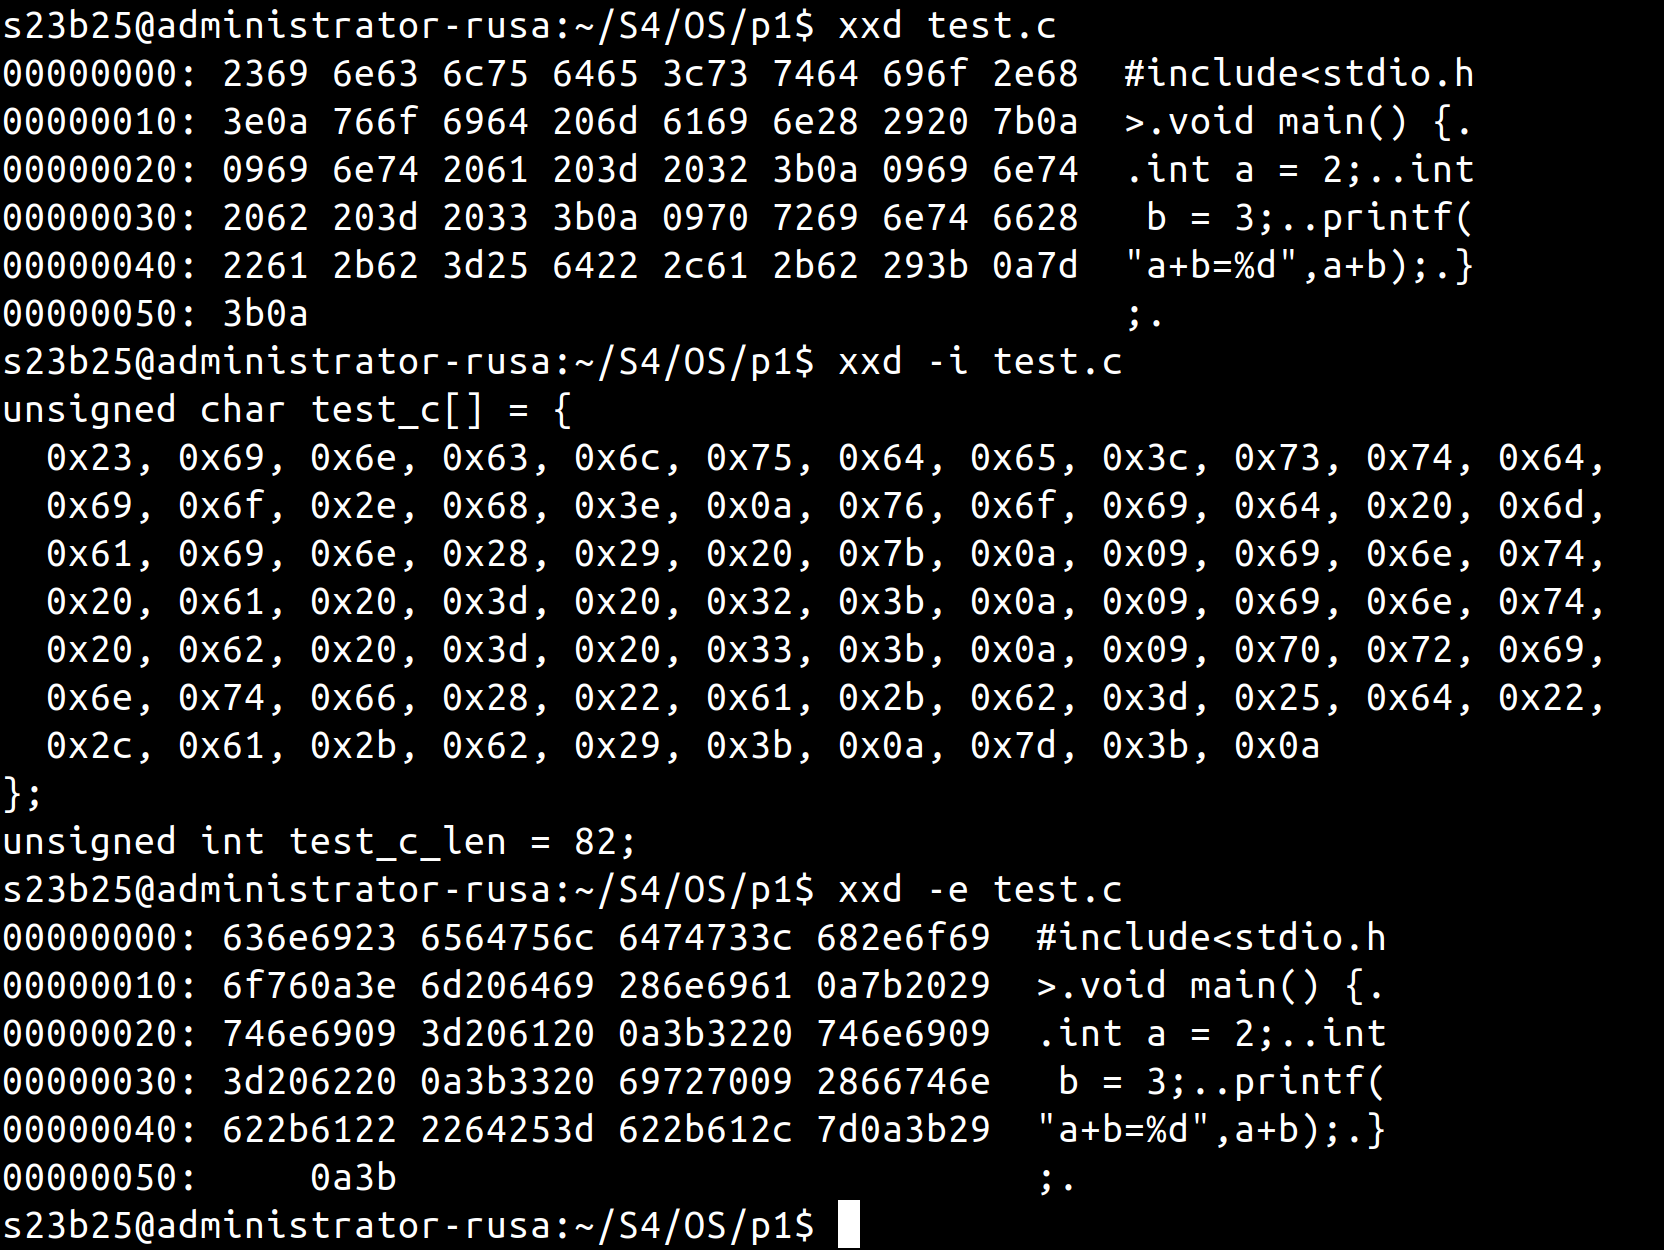
\includegraphics[width=\linewidth]{assets/xxd-1.png}
\end{minipage}
} %output screenshot name
\end{figure}
\subsection{Command 11: fuser} 
\textbf{Purpose}
\begin{flushleft}
       fuser - list process IDs of all processes that have one or more files
\end{flushleft}
\textbf{Usage}
\begin{verbatim}
fuser -l
\end{verbatim}
\textbf{Sample i/p and o/p}
\begin{figure}[H] 
\fbox{
\begin{minipage}{350px} 
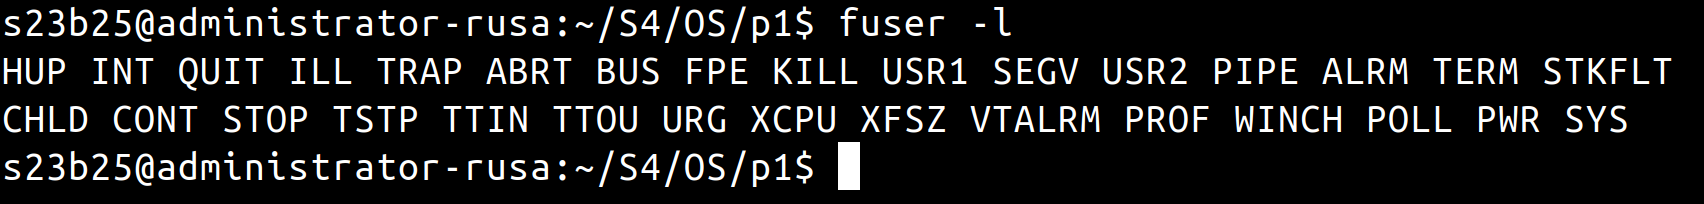
\includegraphics[width=\linewidth]{assets/fuser-1.png}
\end{minipage}
} %output screenshot name
\end{figure}
\subsection{Command 12: top} 
\textbf{Purpose}
\begin{flushleft}
 display sorted information about processes
\end{flushleft}
\textbf{Usage}
\begin{verbatim}
top
\end{verbatim}
\textbf{Sample i/p and o/p}
\begin{figure}[H] 
\fbox{
\begin{minipage}{350px} 
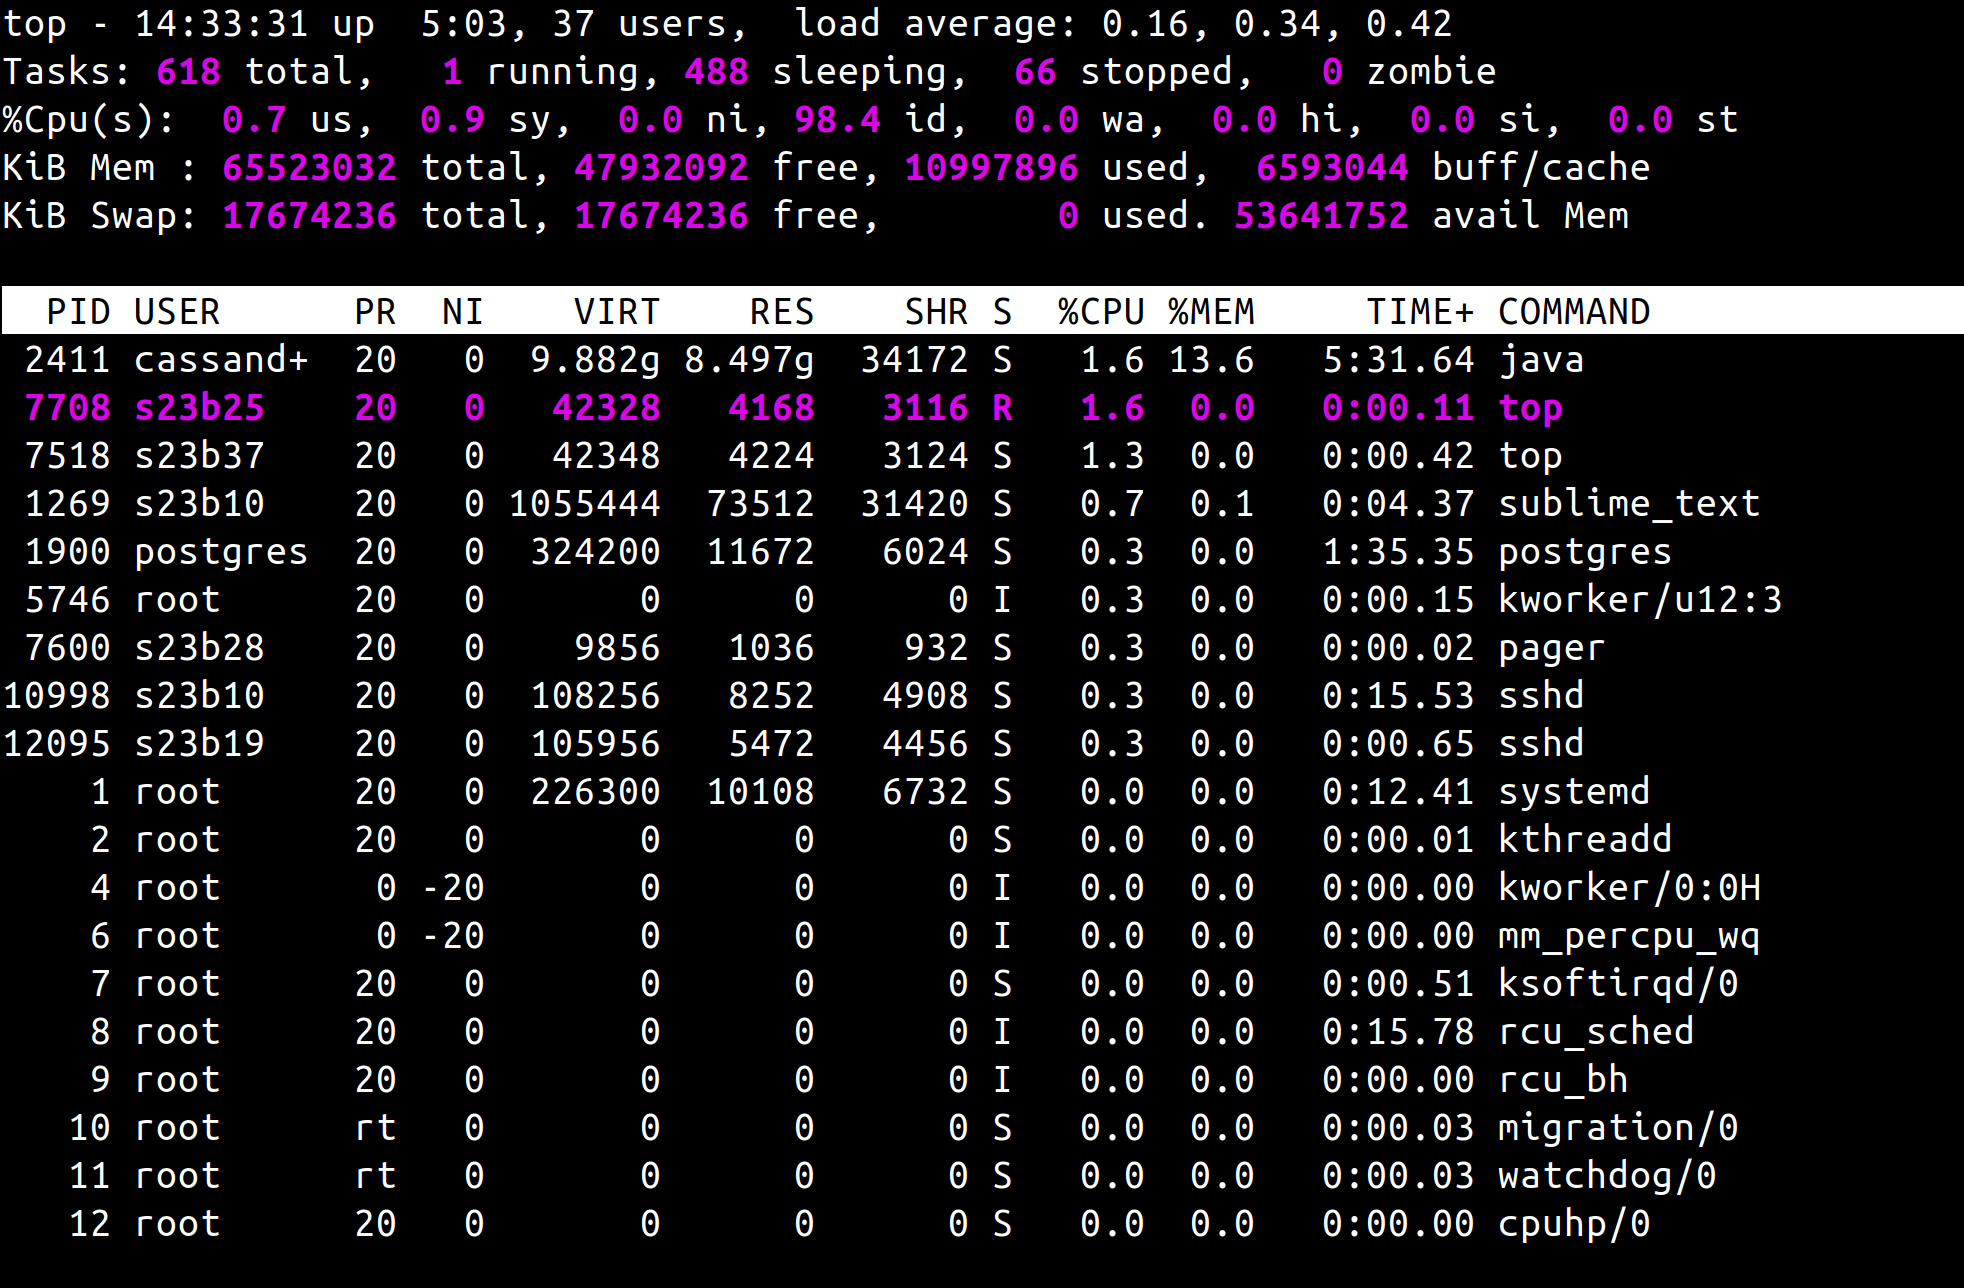
\includegraphics[width=\linewidth]{assets/top-1.png}
\end{minipage}
} %output screenshot name
\end{figure}
\subsection{Command 13: awk} 
\textbf{Purpose}
\begin{flushleft}
       awk - pattern-directed scanning and processing language
\end{flushleft}
\textbf{Usage}
\begin{verbatim}
gawk -F: '{print }' /etc/passwd
\end{verbatim}
\textbf{Sample i/p and o/p}
\begin{figure}[H] 
\fbox{
\begin{minipage}{350px} 
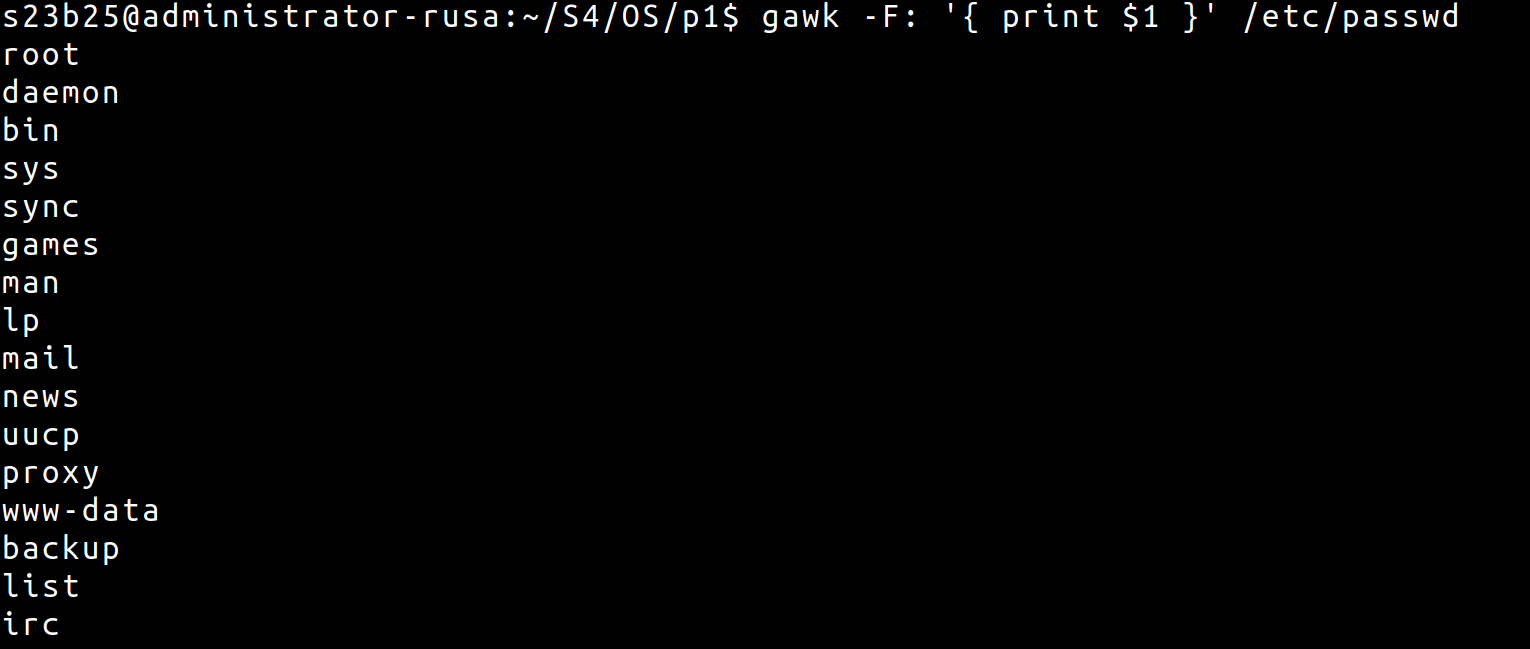
\includegraphics[width=\linewidth]{assets/awk-1.png}
\end{minipage}
} %output screenshot name
\end{figure}
\subsection{Command 14: cal} 
\textbf{Purpose}
\begin{flushleft}
 displays a calendar and the date of Easter
\end{flushleft}
\textbf{Usage}
\begin{verbatim}
cal
cal -j
cal -m 3
\end{verbatim}
\textbf{Sample i/p and o/p}
\begin{figure}[H] 
\fbox{
\begin{minipage}{350px} 
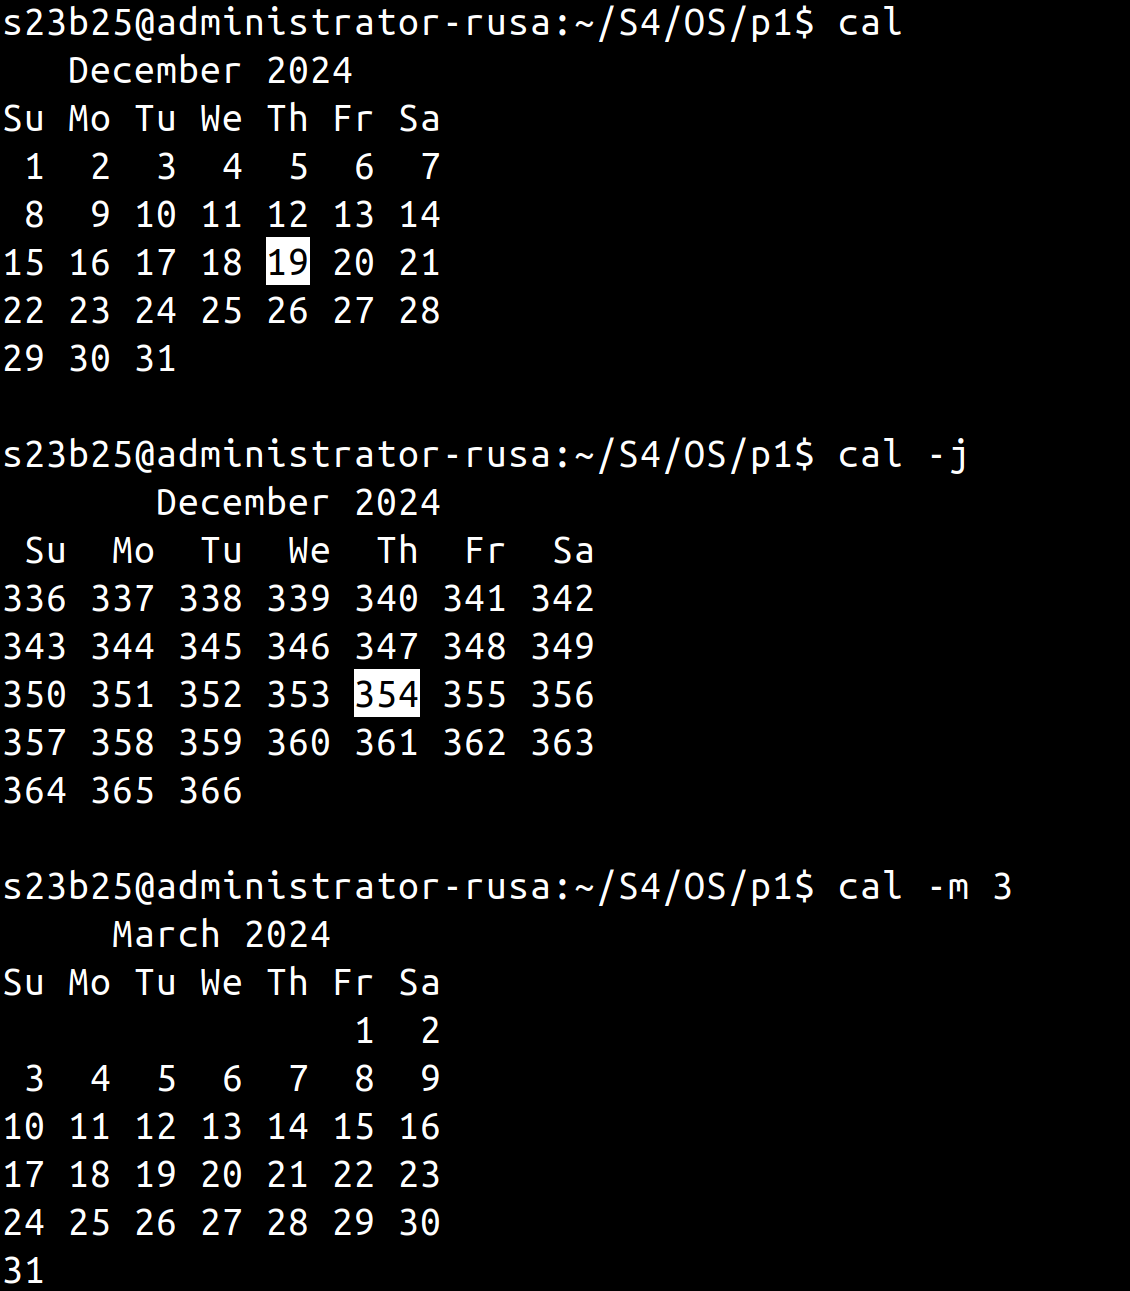
\includegraphics[width=\linewidth]{assets/cal-1.png}
\end{minipage}
} %output screenshot name
\end{figure}
\subsection{Command 15: ls} 
\textbf{Purpose}
\begin{flushleft}
 list directory contents
\end{flushleft}
\textbf{Usage}
\begin{verbatim}
ls
ls -a
ls -l
\end{verbatim}
\textbf{Sample i/p and o/p}
\begin{figure}[H] 
\fbox{
\begin{minipage}{350px} 
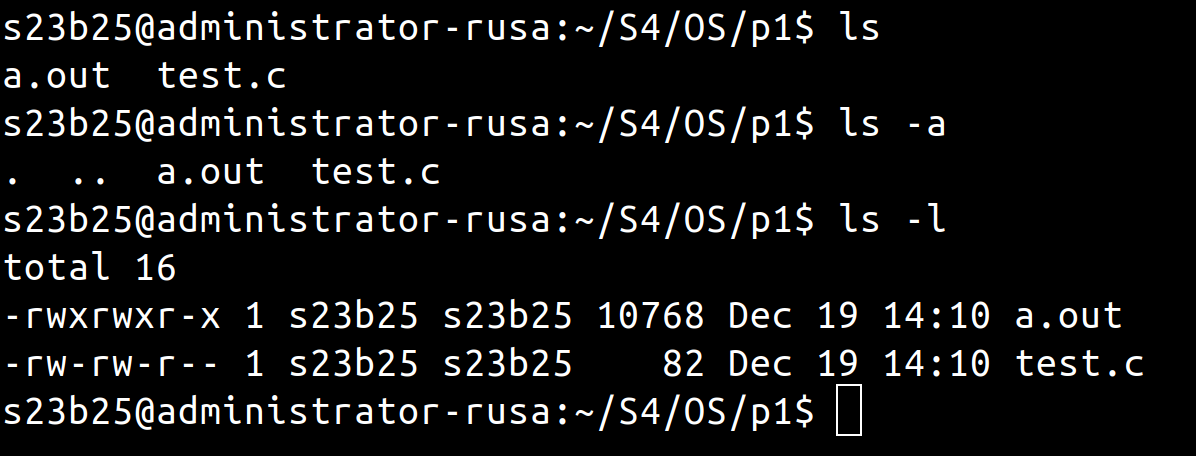
\includegraphics[width=\linewidth]{assets/ls-1.png}
\end{minipage}
} %output screenshot name
\end{figure}
\subsection{Command 16: chmod} 
\textbf{Purpose}
\begin{flushleft}
 change file modes or Access Control Lists
\end{flushleft}
\textbf{Usage}
\begin{verbatim}
chmod +x test.sh
chmod +r test.sh
chmod +w test.sh
\end{verbatim}
\textbf{Sample i/p and o/p}
\begin{figure}[H] 
\fbox{
\begin{minipage}{350px} 
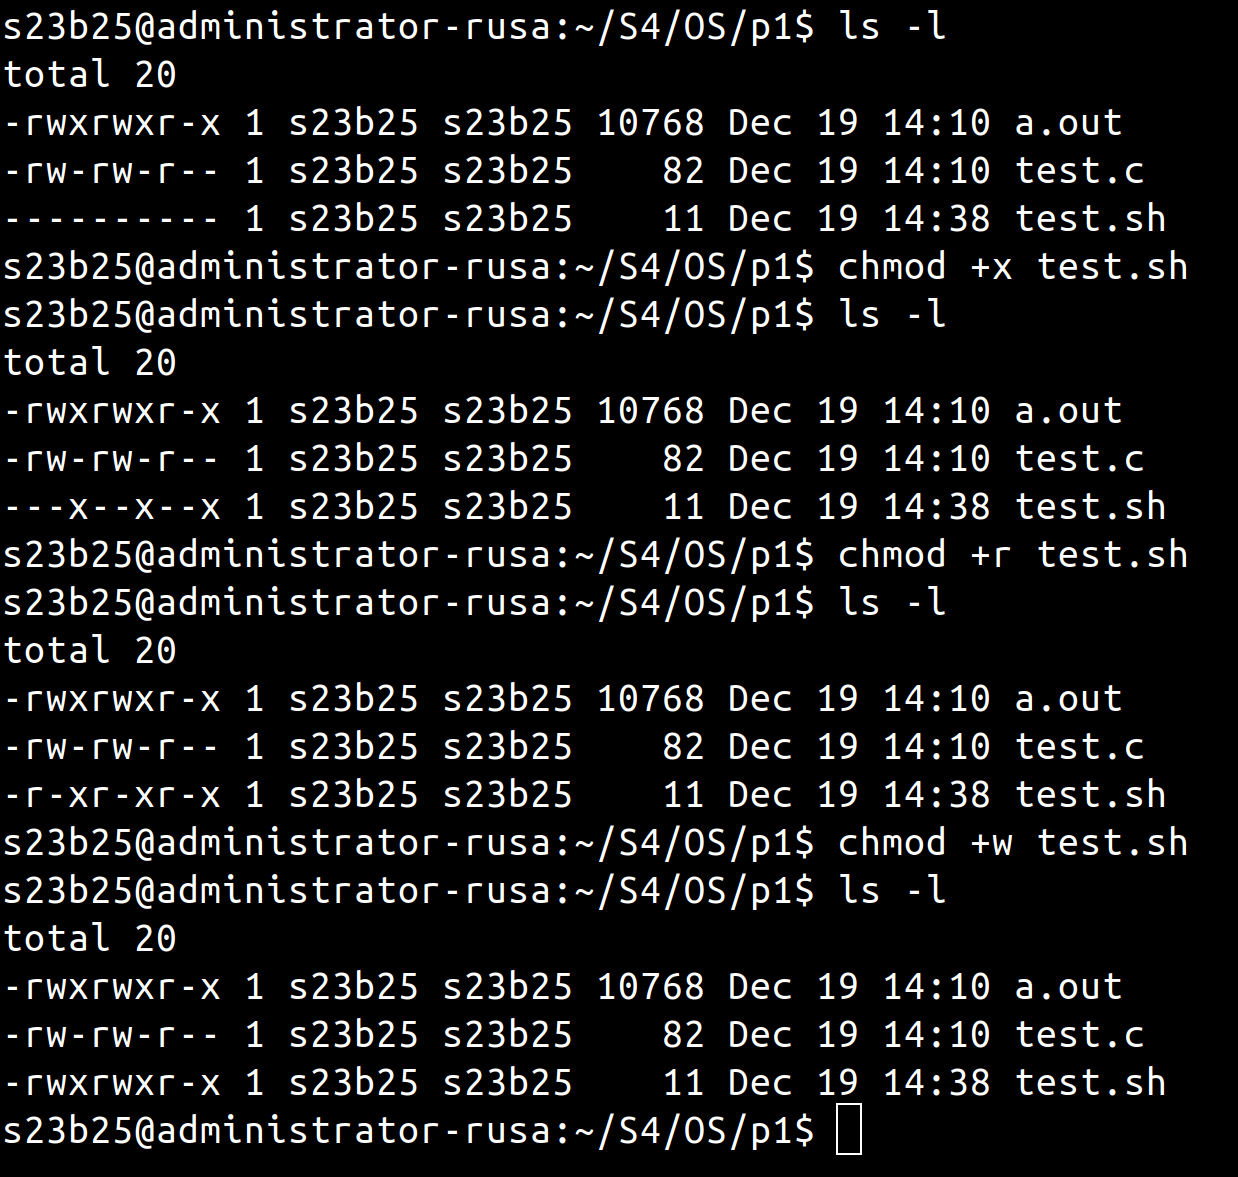
\includegraphics[width=\linewidth]{assets/chmod-1.png}
\end{minipage}
} %output screenshot name
\end{figure}
\subsection{Command 17: chown} 
\textbf{Purpose}
\begin{flushleft}
 change file owner and group
\end{flushleft}
\textbf{Usage}
\begin{verbatim}
%usage%
\end{verbatim}
\textbf{Sample i/p and o/p}
\begin{figure}[H] 
\fbox{
\begin{minipage}{350px} 
\includegraphics[width=\linewidth]{assets/chown-*}
\end{minipage}
} %output screenshot name
\end{figure}
\subsection{Command 18: chgrp} 
\textbf{Purpose}
\begin{flushleft}
 change group
\end{flushleft}
\textbf{Usage}
\begin{verbatim}
%usage%
\end{verbatim}
\textbf{Sample i/p and o/p}
\begin{figure}[H] 
\fbox{
\begin{minipage}{350px} 
\includegraphics[width=\linewidth]{assets/chgrp-*}
\end{minipage}
} %output screenshot name
\end{figure}
\subsection{Command 19: mkdir} 
\textbf{Purpose}
\begin{flushleft}
 make directories
\end{flushleft}
\textbf{Usage}
\begin{verbatim}
mkdir test/
mkdir -p test/nested1/nested2/
\end{verbatim}
\textbf{Sample i/p and o/p}
\begin{figure}[H] 
\fbox{
\begin{minipage}{350px} 
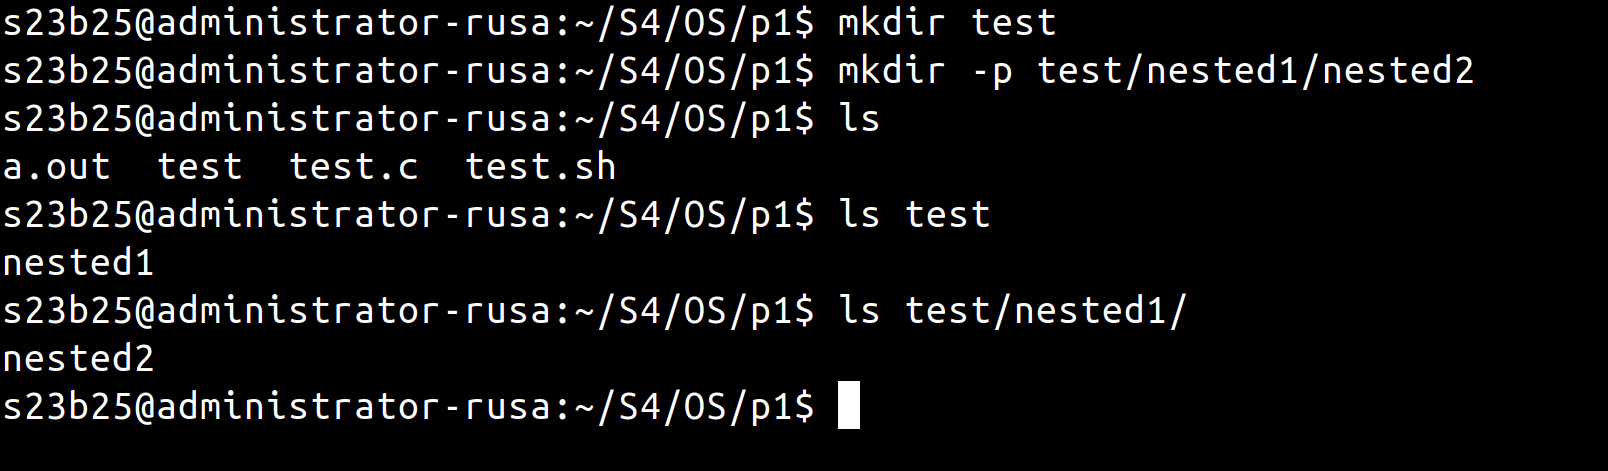
\includegraphics[width=\linewidth]{assets/mkdir-1.png}
\end{minipage}
} %output screenshot name
\end{figure}
\subsection{Command 20: rmdir} 
\textbf{Purpose}
\begin{flushleft}
 remove directories
\end{flushleft}
\textbf{Usage}
\begin{verbatim}
rmdir test/nested1/nested2/
\end{verbatim}
\textbf{Sample i/p and o/p}
\begin{figure}[H] 
\fbox{
\begin{minipage}{350px} 
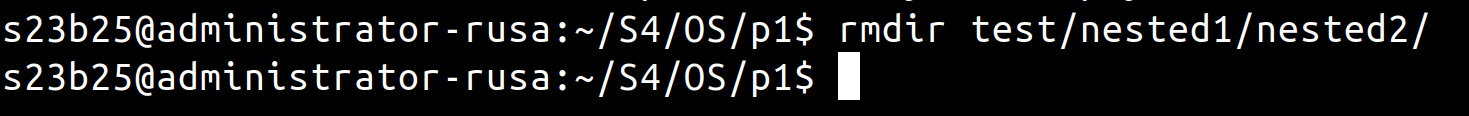
\includegraphics[width=\linewidth]{assets/rmdir-1.png}
\end{minipage}
} %output screenshot name
\end{figure}
\subsection{Command 21: locate} 
\textbf{Purpose}
\begin{flushleft}
 find filenames quickly
\end{flushleft}
\textbf{Usage}
\begin{verbatim}
locate gedit
\end{verbatim}
\textbf{Sample i/p and o/p}
\begin{figure}[H] 
\fbox{
\begin{minipage}{350px} 
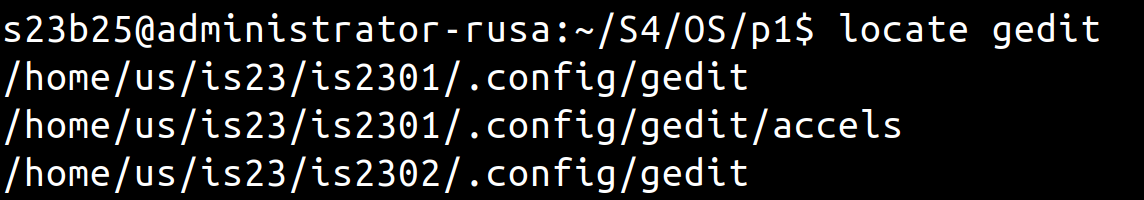
\includegraphics[width=\linewidth]{assets/locate-1.png}
\end{minipage}
} %output screenshot name
\end{figure}
\subsection{Command 22: nftw} 
\textbf{Purpose}
\begin{flushleft}
 traverse (walk) a file tree
\end{flushleft}
\textbf{Usage}
\begin{verbatim}
%usage%
\end{verbatim}
\textbf{Sample i/p and o/p}
\begin{figure}[H] 
\fbox{
\begin{minipage}{350px} 
\includegraphics[width=\linewidth]{assets/nftw-*}
\end{minipage}
} %output screenshot name
\end{figure}
\subsection{Command 23: touch} 
\textbf{Purpose}
\begin{flushleft}
 change file access and modification times
\end{flushleft}
\textbf{Usage}
\begin{verbatim}
touch test.txt
\end{verbatim}
\textbf{Sample i/p and o/p}
\begin{figure}[H] 
\fbox{
\begin{minipage}{350px} 
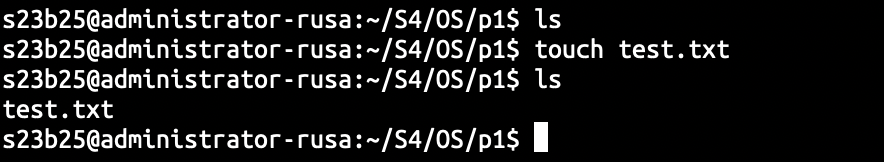
\includegraphics[width=\linewidth]{assets/touch-1.png}
\end{minipage}
} %output screenshot name
\end{figure}
\subsection{Command 24: cat} 
\textbf{Purpose}
\begin{flushleft}
 concatenate and print files
\end{flushleft}
\textbf{Usage}
\begin{verbatim}
cat test.txt
cat -b test.txt
cat -E test.txt
\end{verbatim}
\textbf{Sample i/p and o/p}
\begin{figure}[H] 
\fbox{
\begin{minipage}{350px} 
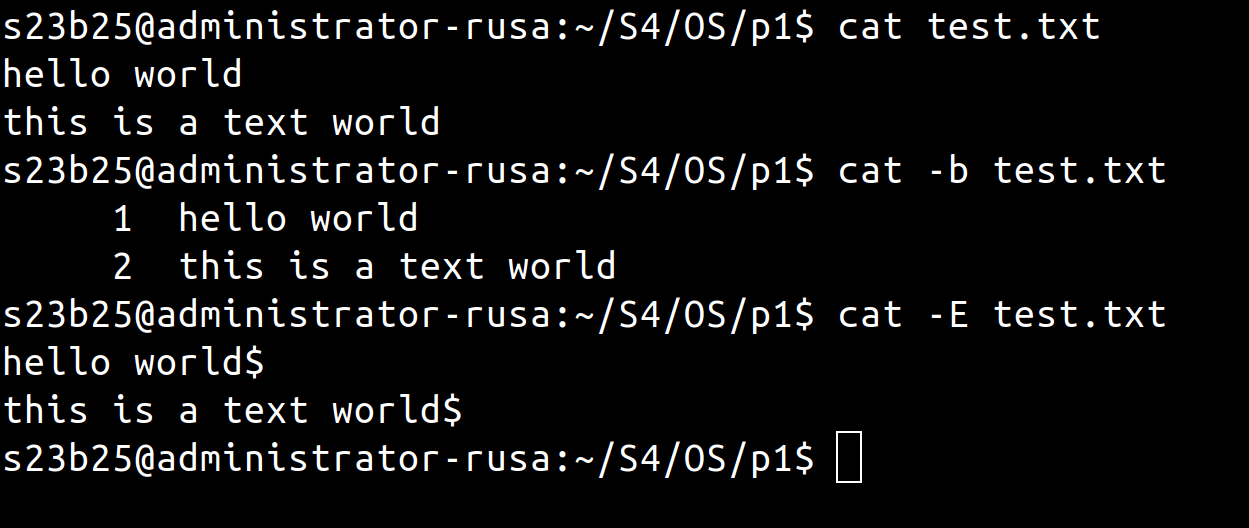
\includegraphics[width=\linewidth]{assets/cat-1.png}
\end{minipage}
} %output screenshot name
\end{figure}
\subsection{Command 25: more} 
\textbf{Purpose}
\begin{flushleft}
       less - opposite of more
\end{flushleft}
\textbf{Usage}
\begin{verbatim}
more test.txt
\end{verbatim}
\textbf{Sample i/p and o/p}
\begin{figure}[H] 
\fbox{
\begin{minipage}{350px} 
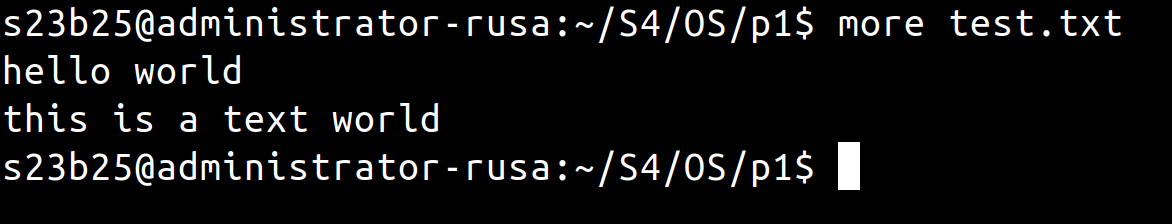
\includegraphics[width=\linewidth]{assets/more-1.png}
\end{minipage}
} %output screenshot name
\end{figure}
\subsection{Command 26: less} 
\textbf{Purpose}
\begin{flushleft}
       less - opposite of more
\end{flushleft}
\textbf{Usage}
\begin{verbatim}
less test.txt
\end{verbatim}
\textbf{Sample i/p and o/p}
\begin{figure}[H] 
\fbox{
\begin{minipage}{350px} 
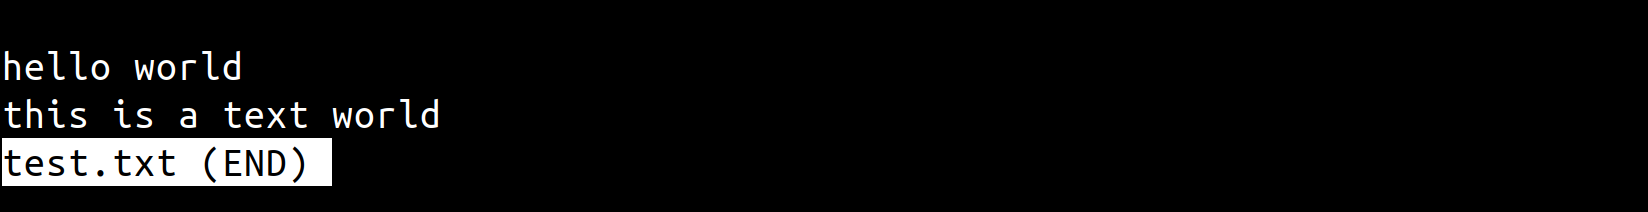
\includegraphics[width=\linewidth]{assets/less-1.png}
\end{minipage}
} %output screenshot name
\end{figure}
\subsection{Command 27: cp} 
\textbf{Purpose}
\begin{flushleft}
 copy files
\end{flushleft}
\textbf{Usage}
\begin{verbatim}
cp test.txt dest/
\end{verbatim}
\textbf{Sample i/p and o/p}
\begin{figure}[H] 
\fbox{
\begin{minipage}{350px} 
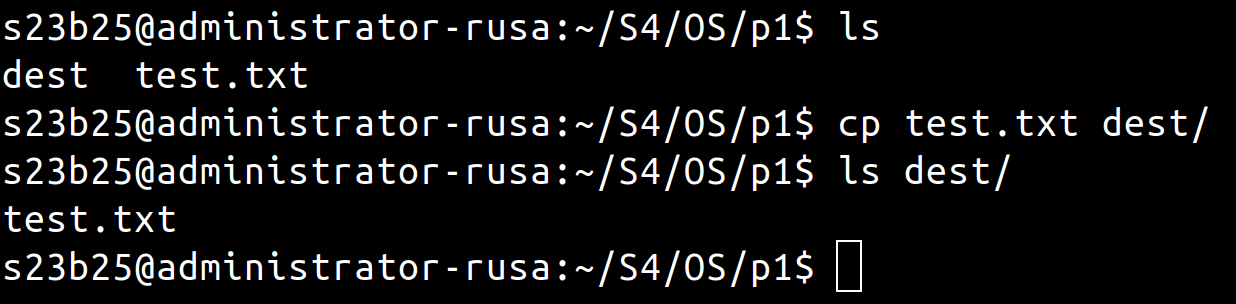
\includegraphics[width=\linewidth]{assets/cp-1.png}
\end{minipage}
} %output screenshot name
\end{figure}
\subsection{Command 28: mv} 
\textbf{Purpose}
\begin{flushleft}
 move files
\end{flushleft}
\textbf{Usage}
\begin{verbatim}
mv src/test.txt .
\end{verbatim}
\textbf{Sample i/p and o/p}
\begin{figure}[H] 
\fbox{
\begin{minipage}{350px} 
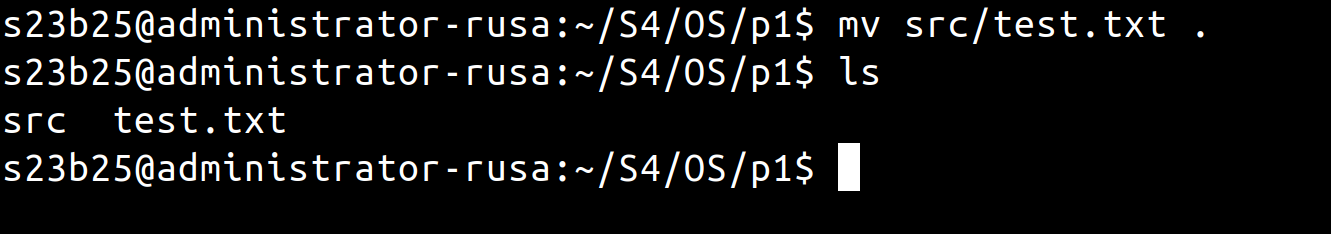
\includegraphics[width=\linewidth]{assets/mv-1.png}
\end{minipage}
} %output screenshot name
\end{figure}
\subsection{Command 29: rm} 
\textbf{Purpose}
\begin{flushleft}
 remove directory entries
\end{flushleft}
\textbf{Usage}
\begin{verbatim}
rm test.txt
\end{verbatim}
\textbf{Sample i/p and o/p}
\begin{figure}[H] 
\fbox{
\begin{minipage}{350px} 
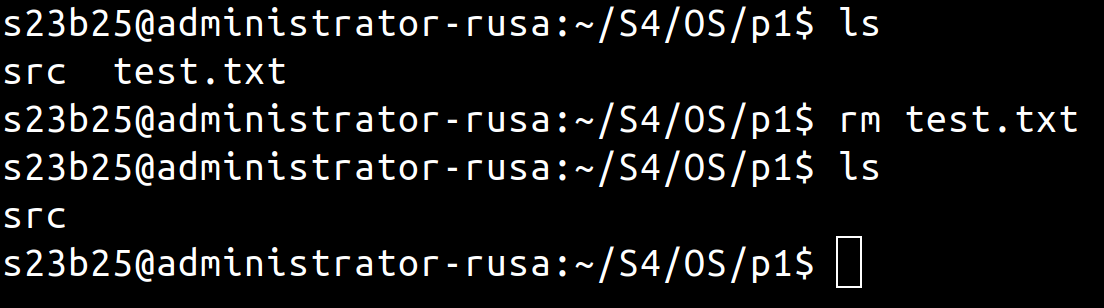
\includegraphics[width=\linewidth]{assets/rm-1.png}
\end{minipage}
} %output screenshot name
\end{figure}
\subsection{Command 30: grep} 
\textbf{Purpose}
\begin{flushleft}
     ggrreepp, eeggrreepp, ffggrreepp, rrggrreepp, bbzzggrreepp, bbzzeeggrreepp, bbzzffggrreepp, zzggrreepp, zzeeggrreepp,
\end{flushleft}
\textbf{Usage}
\begin{verbatim}
man grep | grep description
\end{verbatim}
\textbf{Sample i/p and o/p}
\begin{figure}[H] 
\fbox{
\begin{minipage}{350px} 
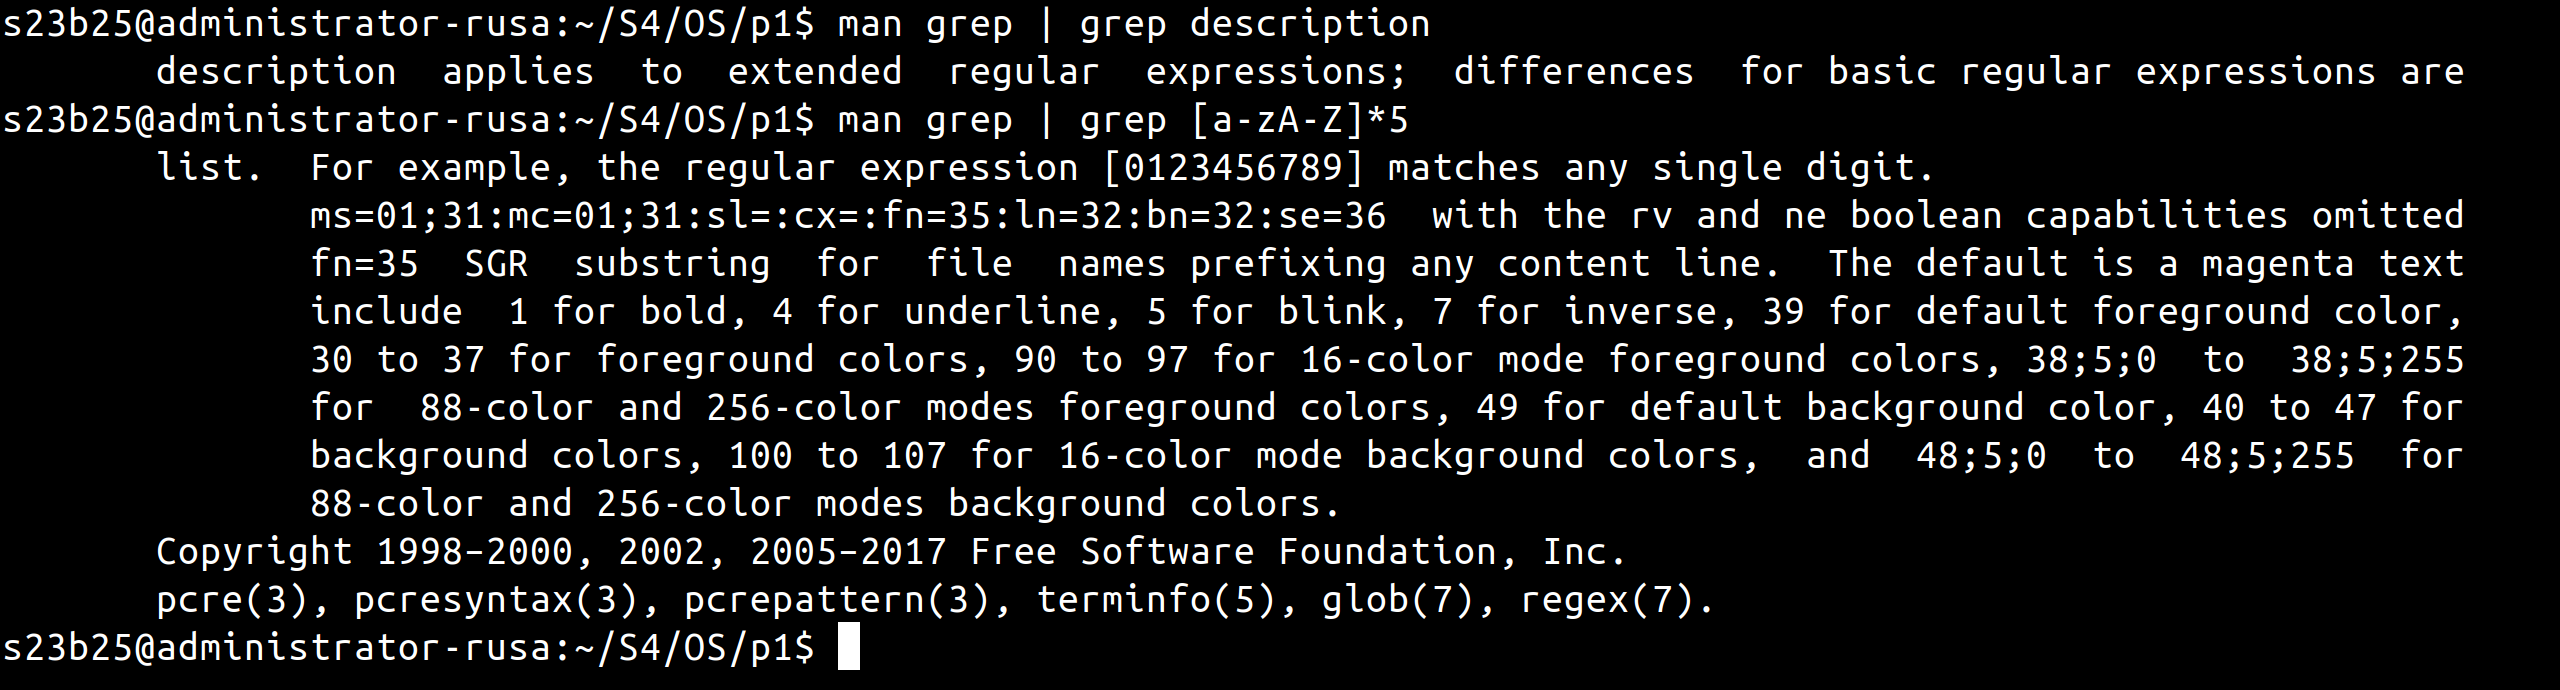
\includegraphics[width=\linewidth]{assets/grep-1.png}
\end{minipage}
} %output screenshot name
\end{figure}
\subsection{Command 31: tail} 
\textbf{Purpose}
\begin{flushleft}
 display the last part of a file
\end{flushleft}
\textbf{Usage}
\begin{verbatim}
tail test.txt
tail test.txt -n 4
tail test.txt -c 10
\end{verbatim}
\textbf{Sample i/p and o/p}
\begin{figure}[H] 
\fbox{
\begin{minipage}{350px} 
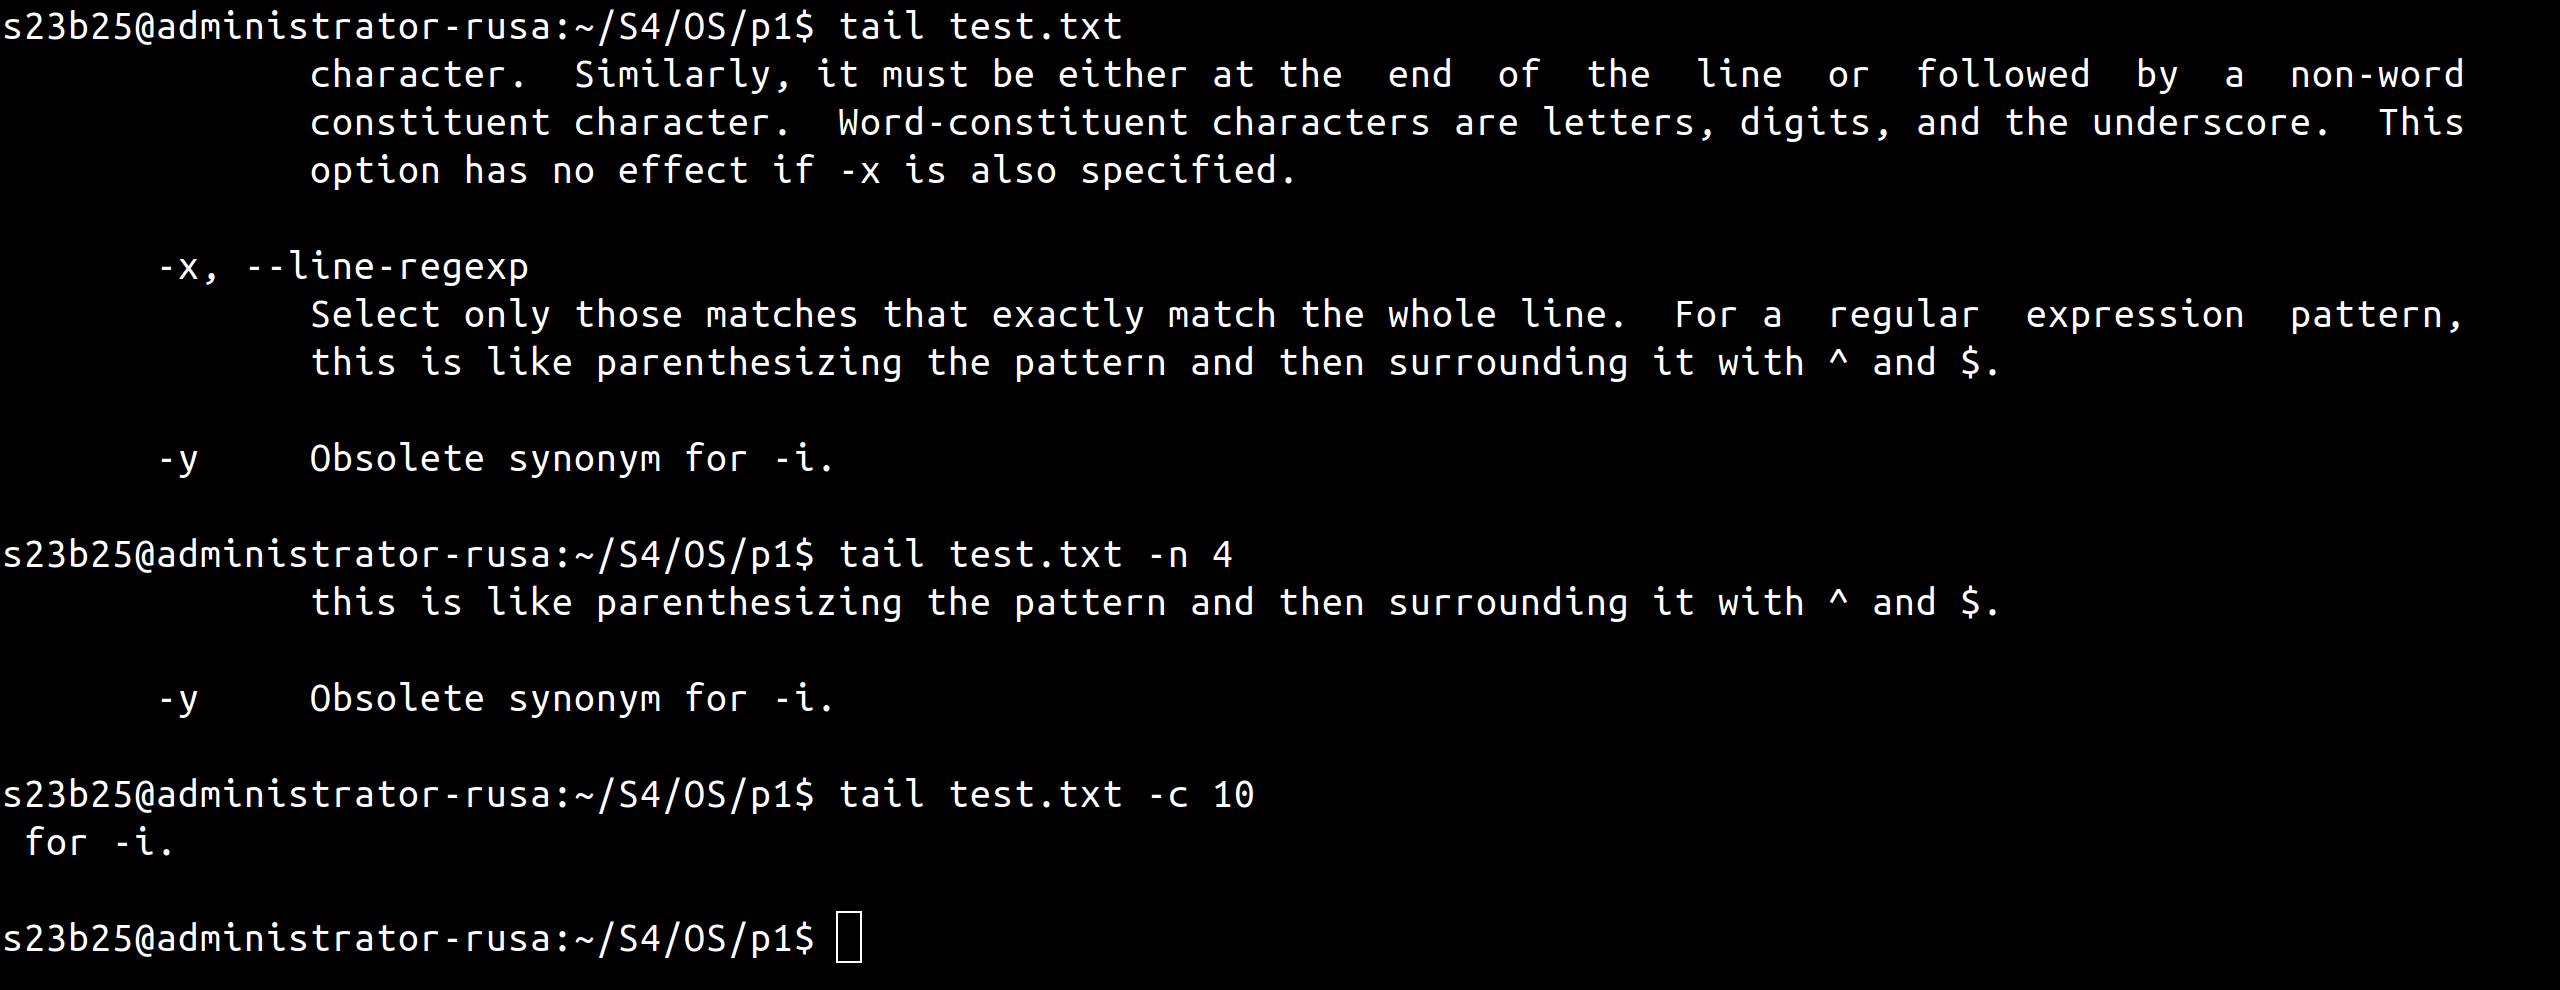
\includegraphics[width=\linewidth]{assets/tail-1.png}
\end{minipage}
} %output screenshot name
\end{figure}
\subsection{Command 32: head} 
\textbf{Purpose}
\begin{flushleft}
 display first lines of a file
\end{flushleft}
\textbf{Usage}
\begin{verbatim}
head test.txt
head test.txt -n 4
head test.txt -c 10
\end{verbatim}
\textbf{Sample i/p and o/p}
\begin{figure}[H] 
\fbox{
\begin{minipage}{350px} 
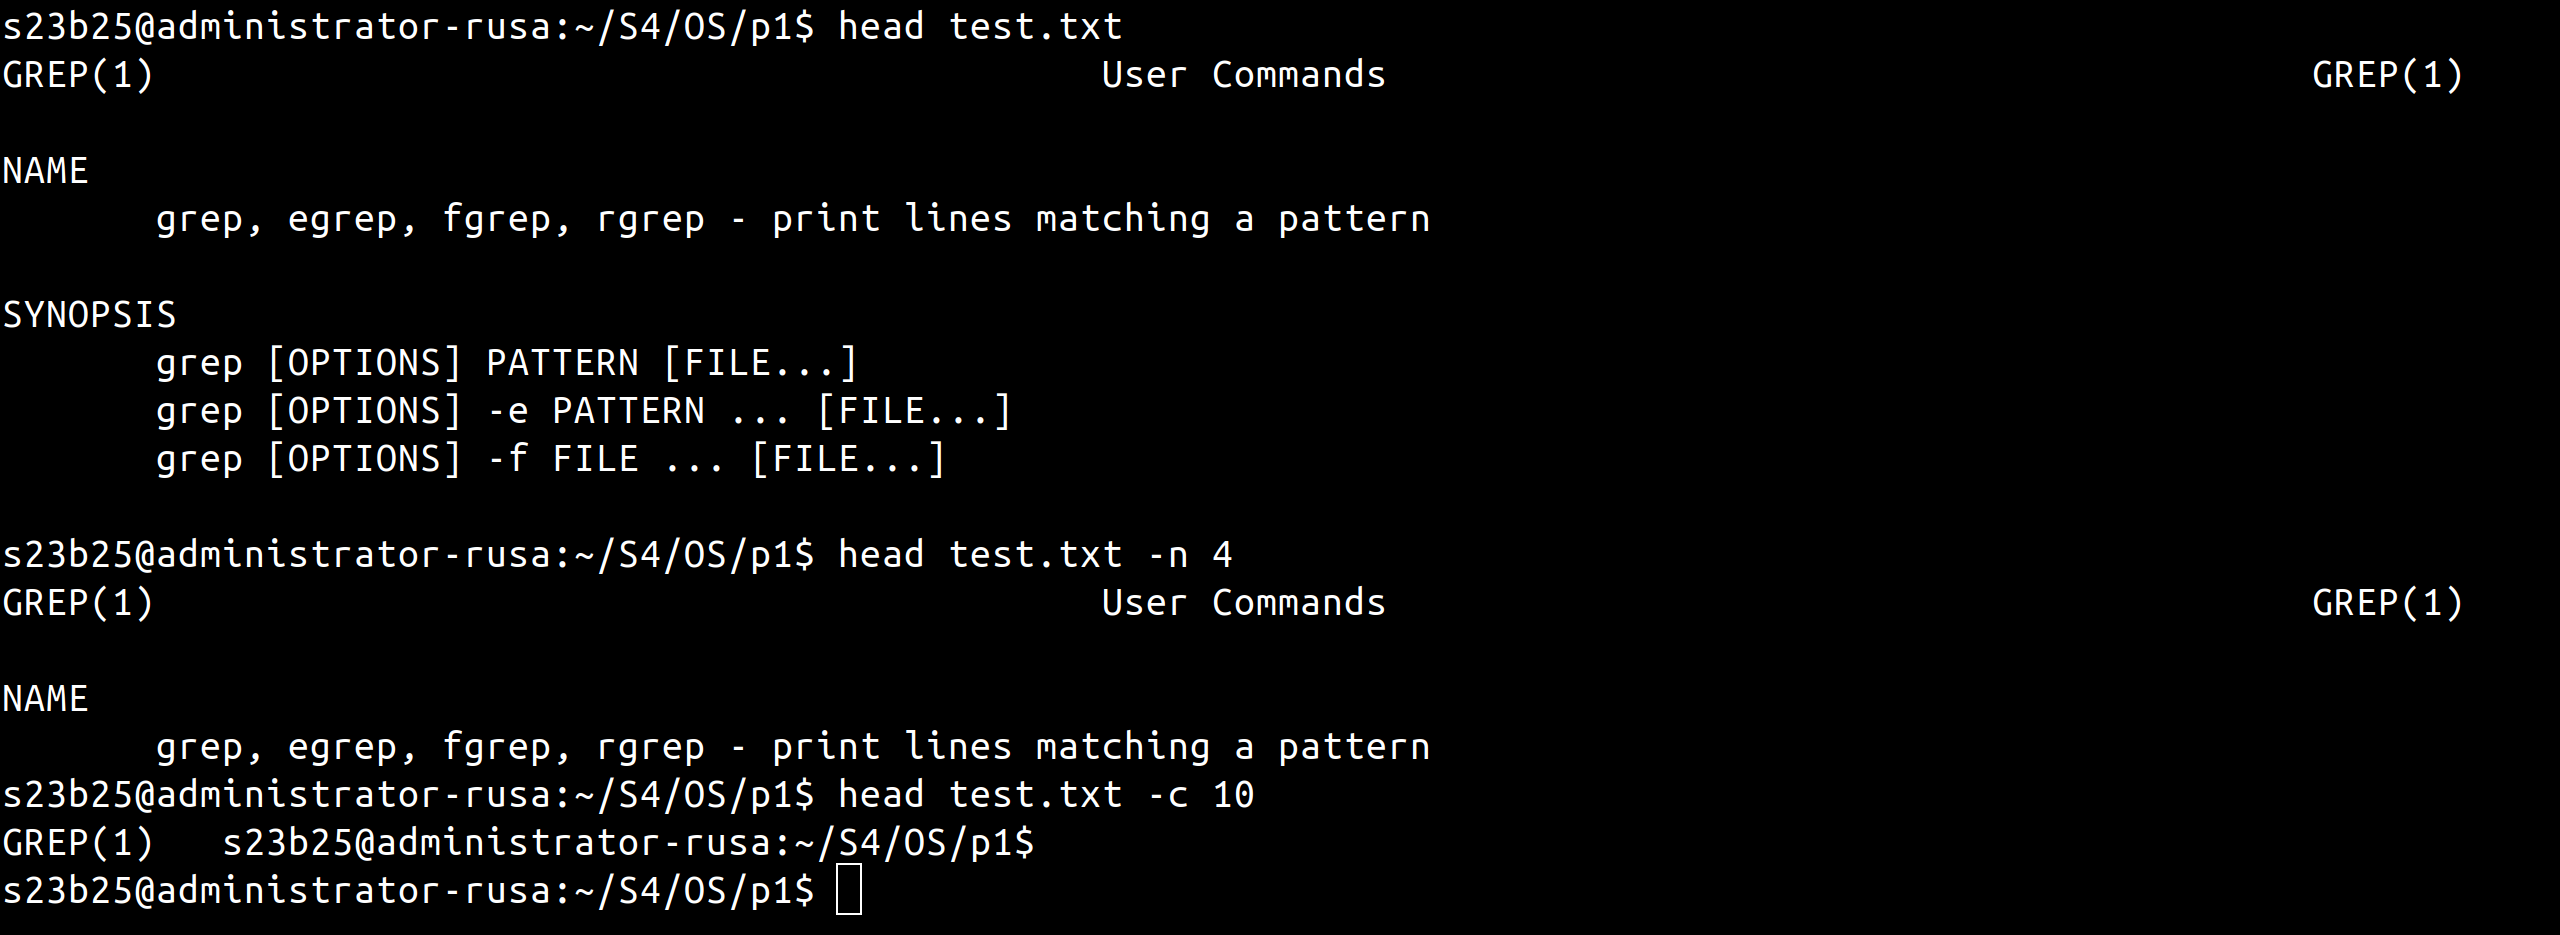
\includegraphics[width=\linewidth]{assets/head-1.png}
\end{minipage}
} %output screenshot name
\end{figure}
\subsection{Command 33: find} 
\textbf{Purpose}
\begin{flushleft}
 walk a file hierarchy
\end{flushleft}
\textbf{Usage}
\begin{verbatim}
find world.c
\end{verbatim}
\textbf{Sample i/p and o/p}
\begin{figure}[H] 
\fbox{
\begin{minipage}{350px} 
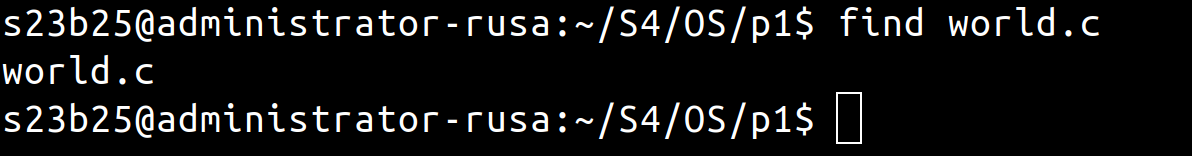
\includegraphics[width=\linewidth]{assets/find-1.png}
\end{minipage}
} %output screenshot name
\end{figure}
\subsection{Command 34: sort} 
\textbf{Purpose}
\begin{flushleft}
 sort or merge records (lines) of text and binary files
\end{flushleft}
\textbf{Usage}
\begin{verbatim}
sort test.txt
sort -r test.txt
\end{verbatim}
\textbf{Sample i/p and o/p}
\begin{figure}[H] 
\fbox{
\begin{minipage}{350px} 
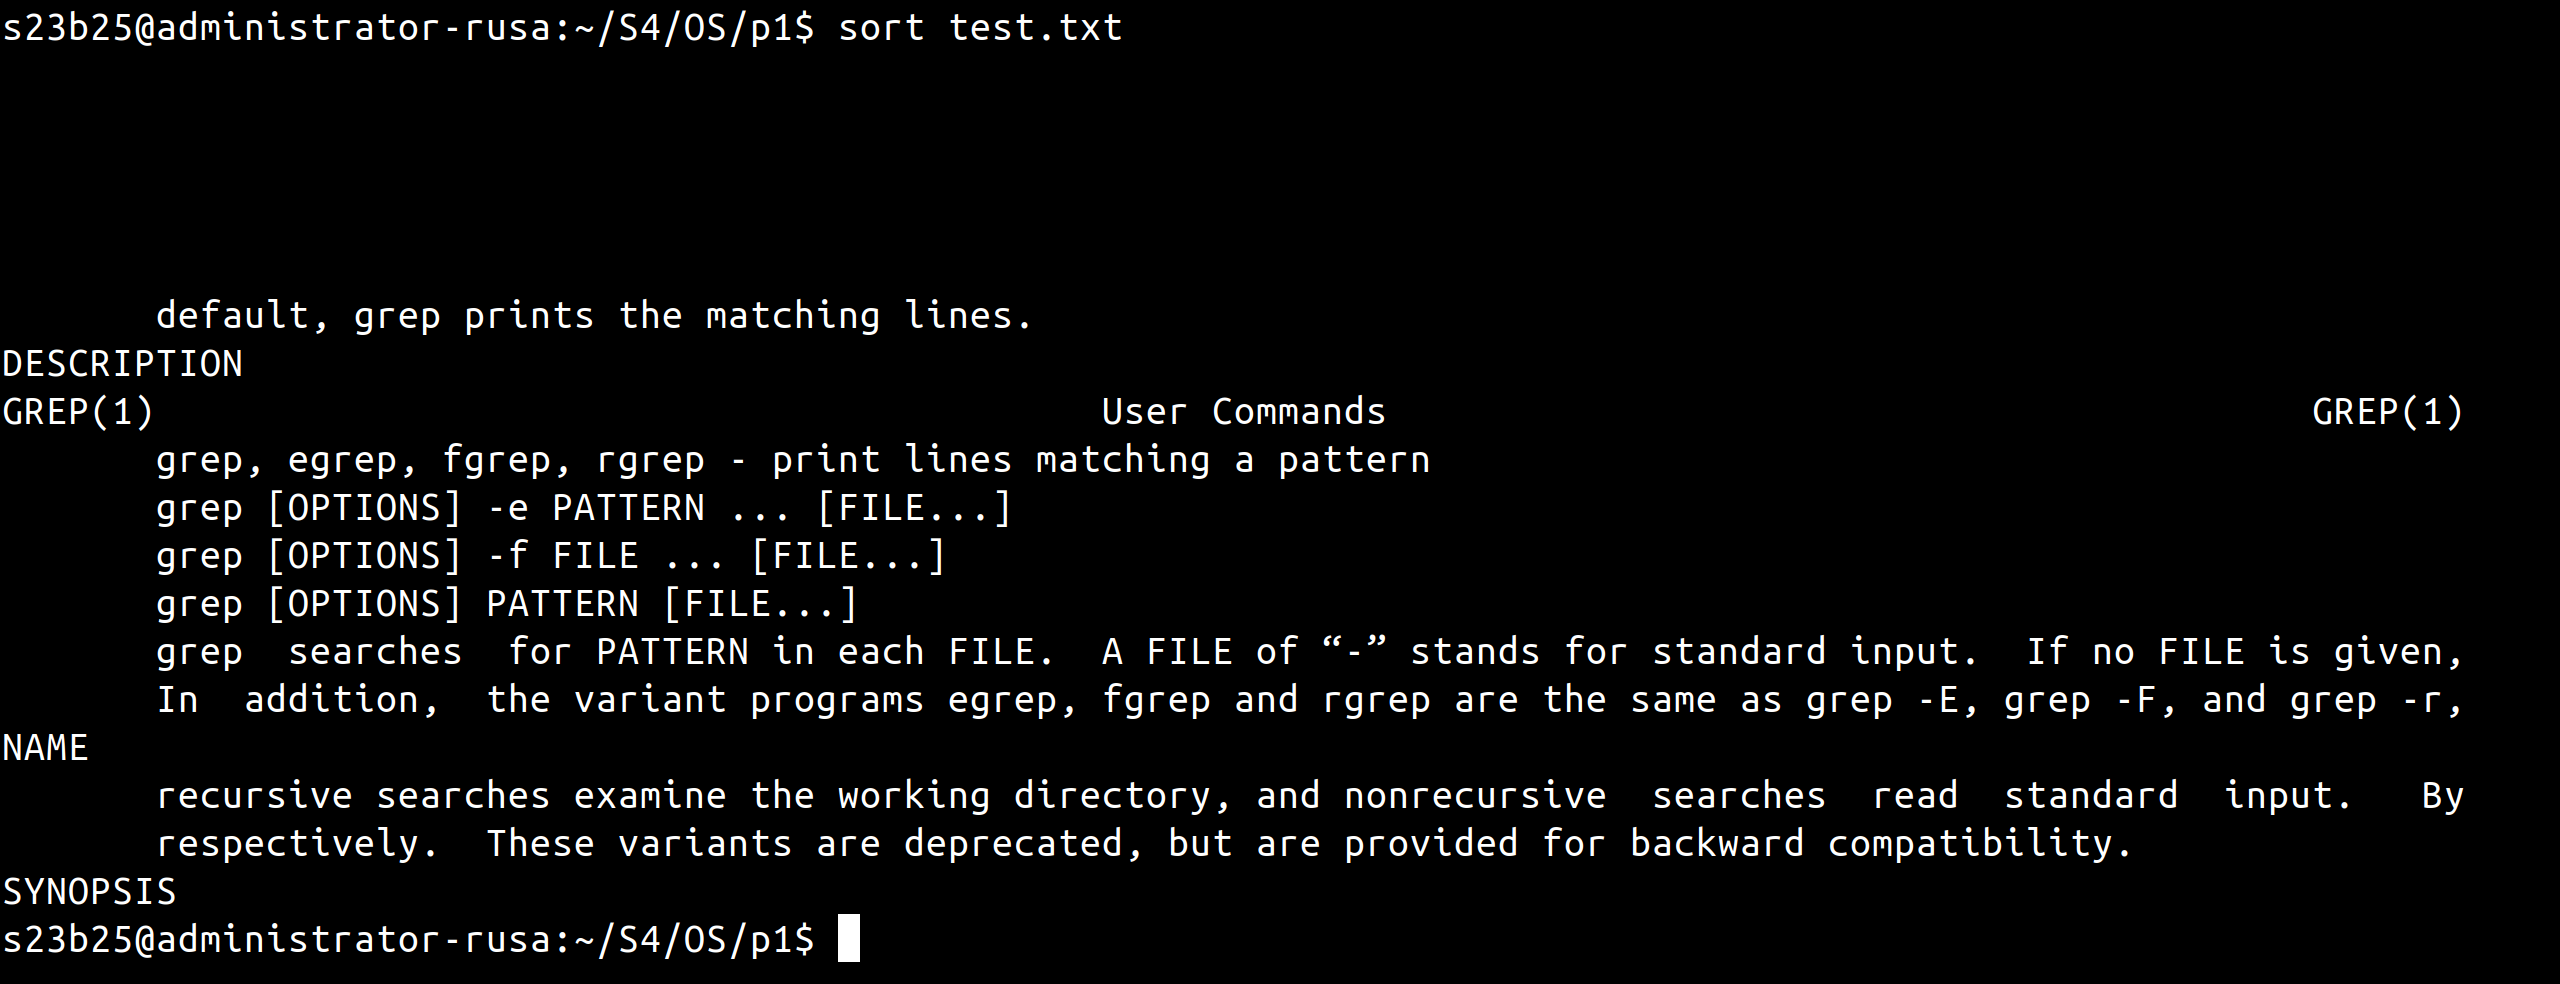
\includegraphics[width=\linewidth]{assets/sort-1.png}
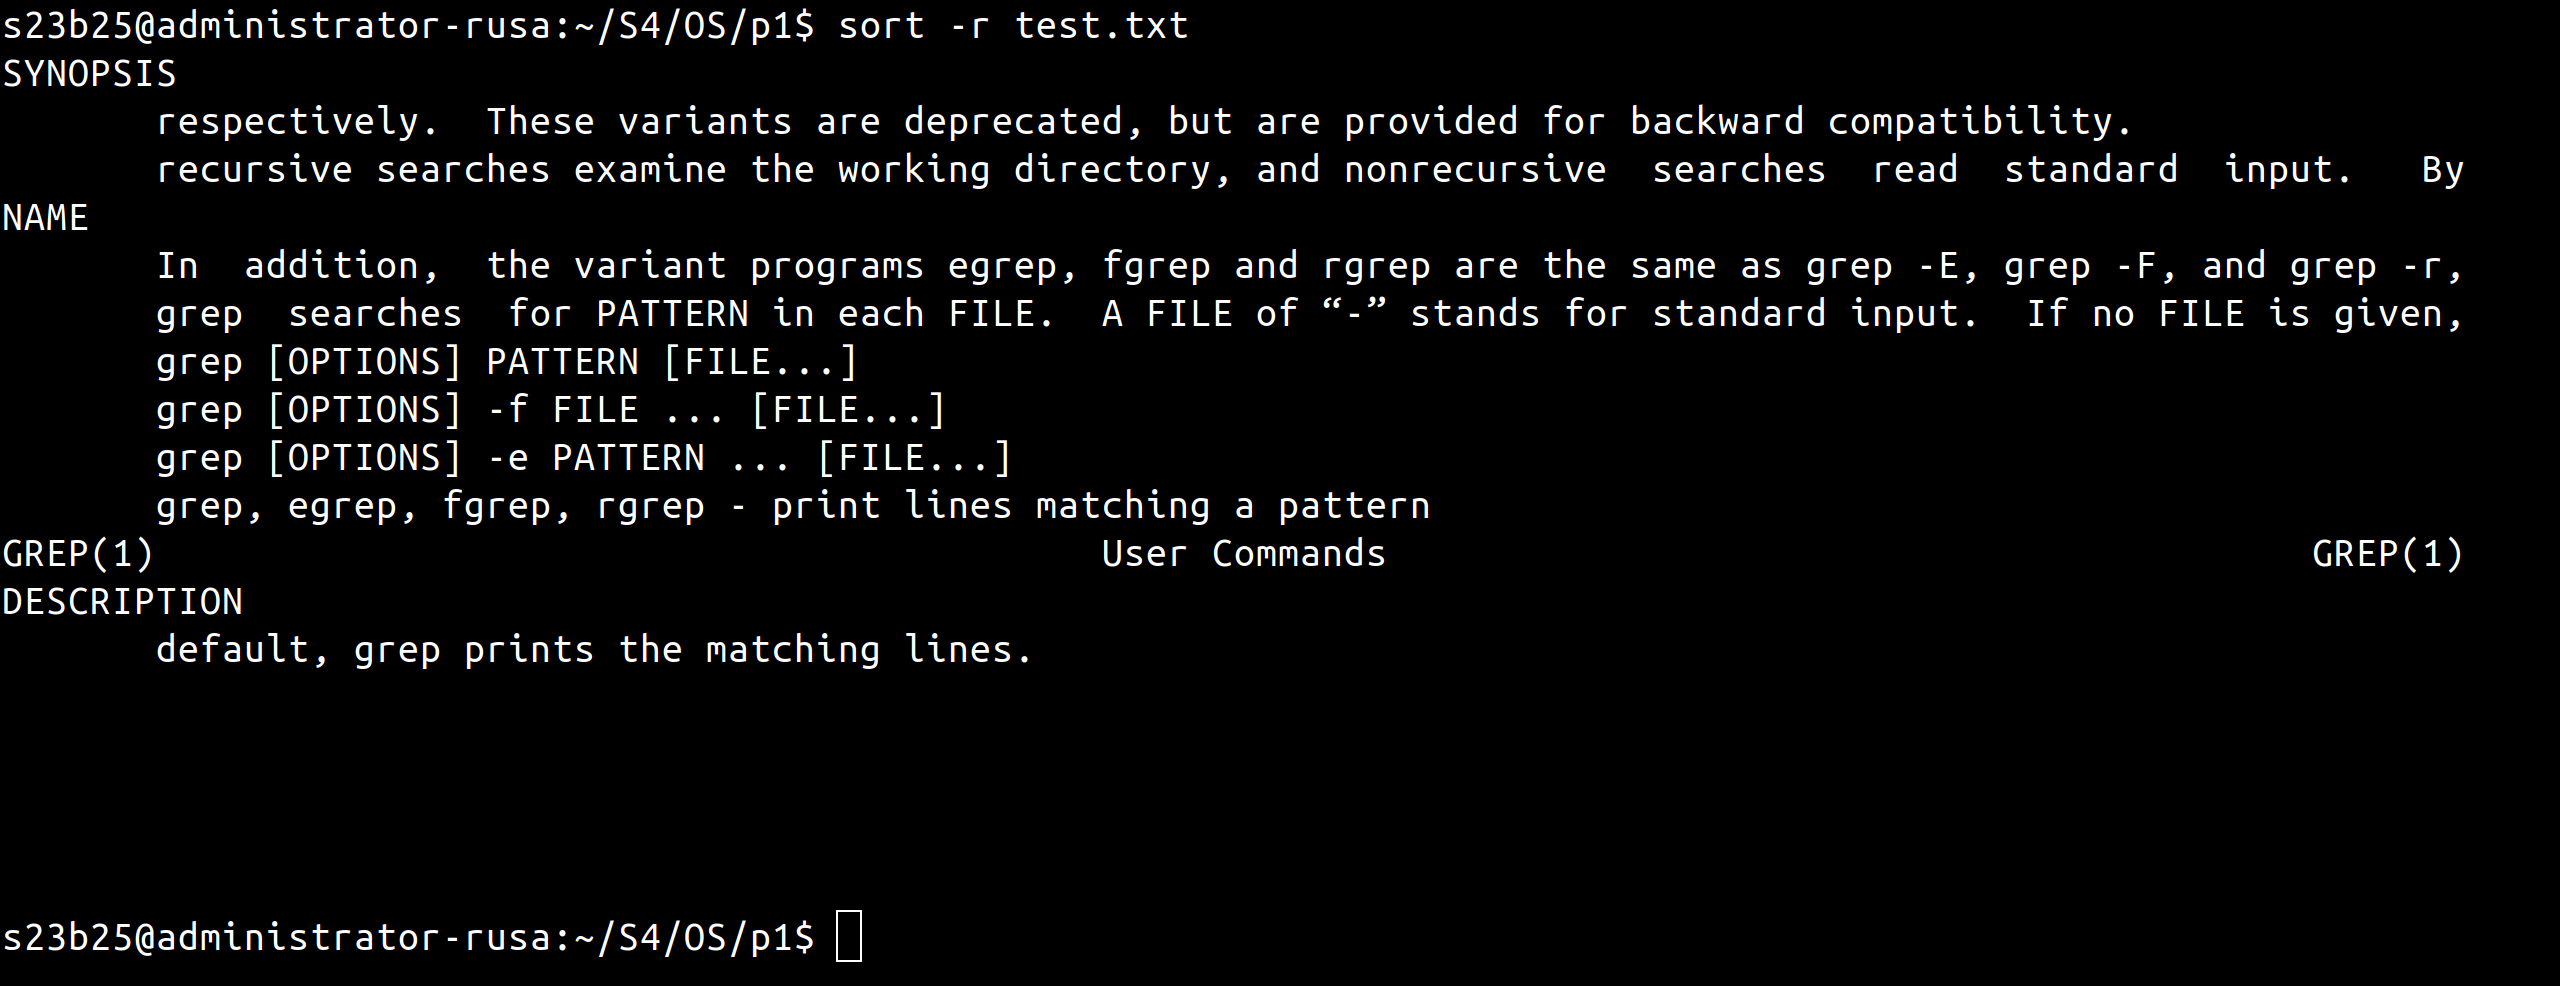
\includegraphics[width=\linewidth]{assets/sort-2.png}
\end{minipage}
} %output screenshot name
\end{figure}
\subsection{Command 35: stty} 
\textbf{Purpose}
\begin{flushleft}
 set the options for a terminal device interface
\end{flushleft}
\textbf{Usage}
\begin{verbatim}
stty
stty -a
\end{verbatim}
\textbf{Sample i/p and o/p}
\begin{figure}[H] 
\fbox{
\begin{minipage}{350px} 
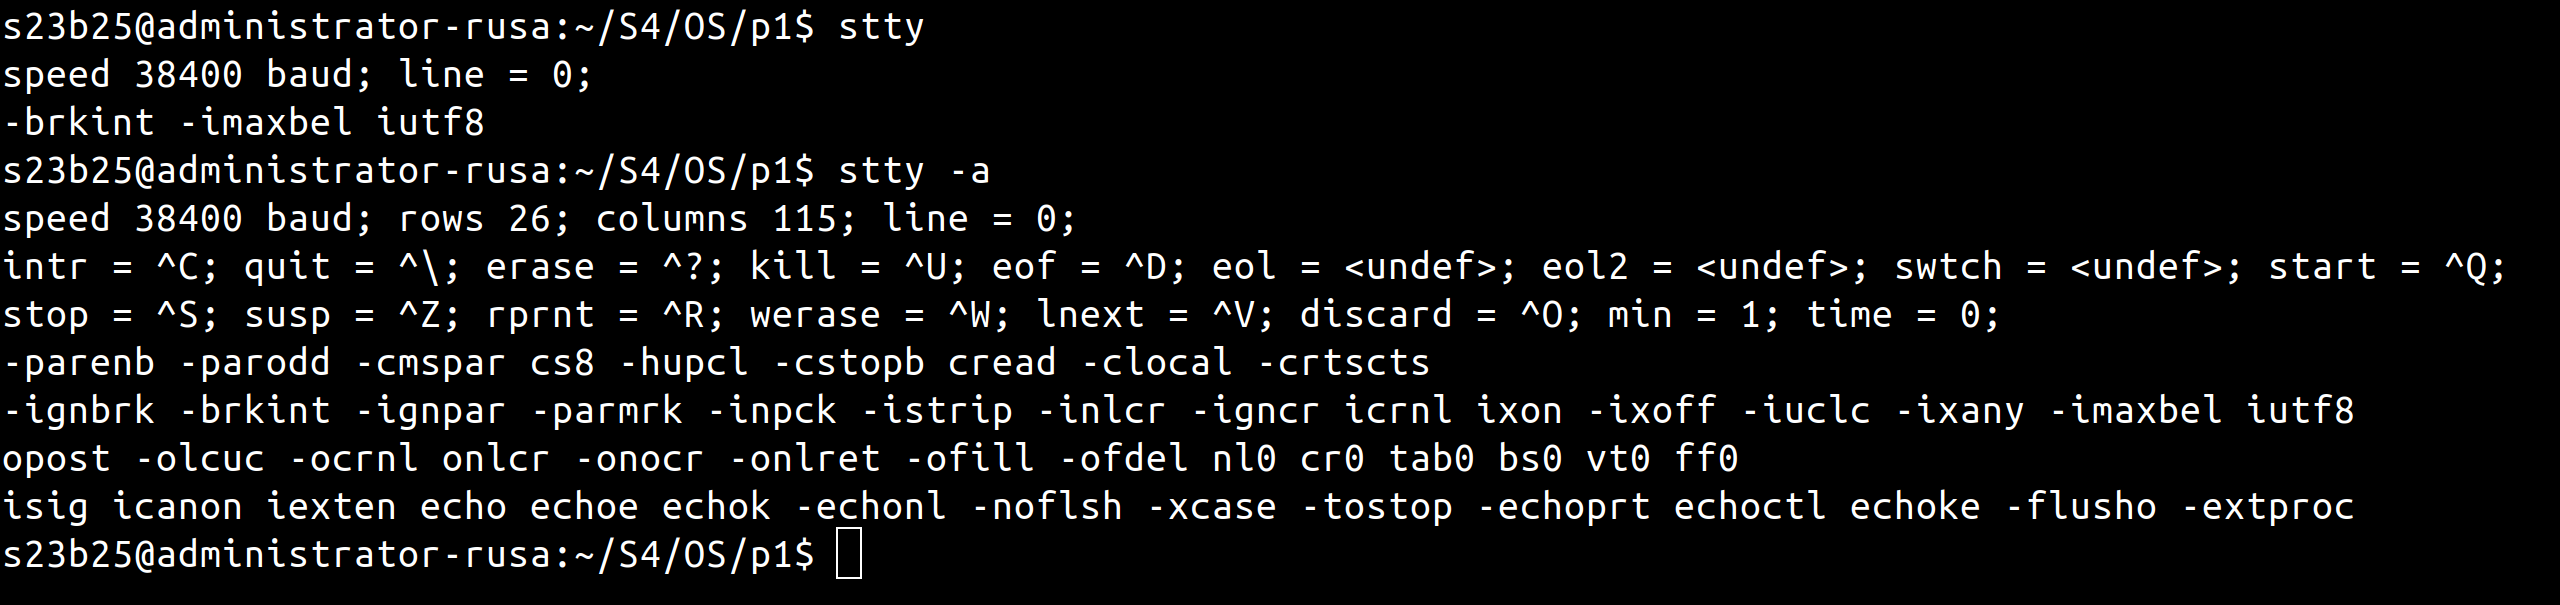
\includegraphics[width=\linewidth]{assets/stty-1.png}
\end{minipage}
} %output screenshot name
\end{figure}
\subsection{Command 36: sed} 
\textbf{Purpose}
\begin{flushleft}
 stream editor
\end{flushleft}
\textbf{Usage}
\begin{verbatim}
sed 's/a/b/g' test.txt
\end{verbatim}
\textbf{Sample i/p and o/p}
\begin{figure}[H] 
\fbox{
\begin{minipage}{350px} 
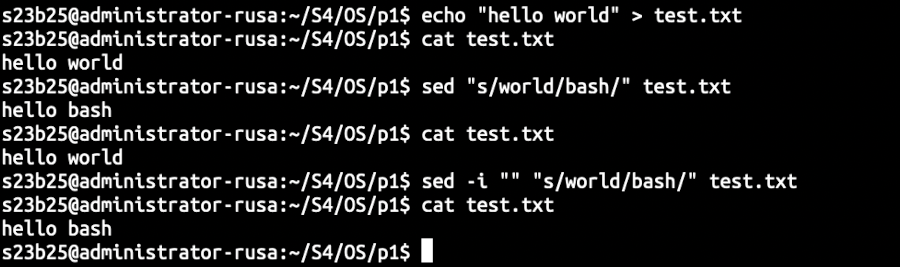
\includegraphics[width=\linewidth]{assets/sed-1.png}
\end{minipage}
} %output screenshot name
\end{figure}
\subsection{Command 37: uniq} 
\textbf{Purpose}
\begin{flushleft}
 report or filter out repeated lines in a file
\end{flushleft}
\textbf{Usage}
\begin{verbatim}
uniq test.txt
uniq test.txt -c
uniq test.txt -d
\end{verbatim}
\textbf{Sample i/p and o/p}
\begin{figure}[H] 
\fbox{
\begin{minipage}{350px} 
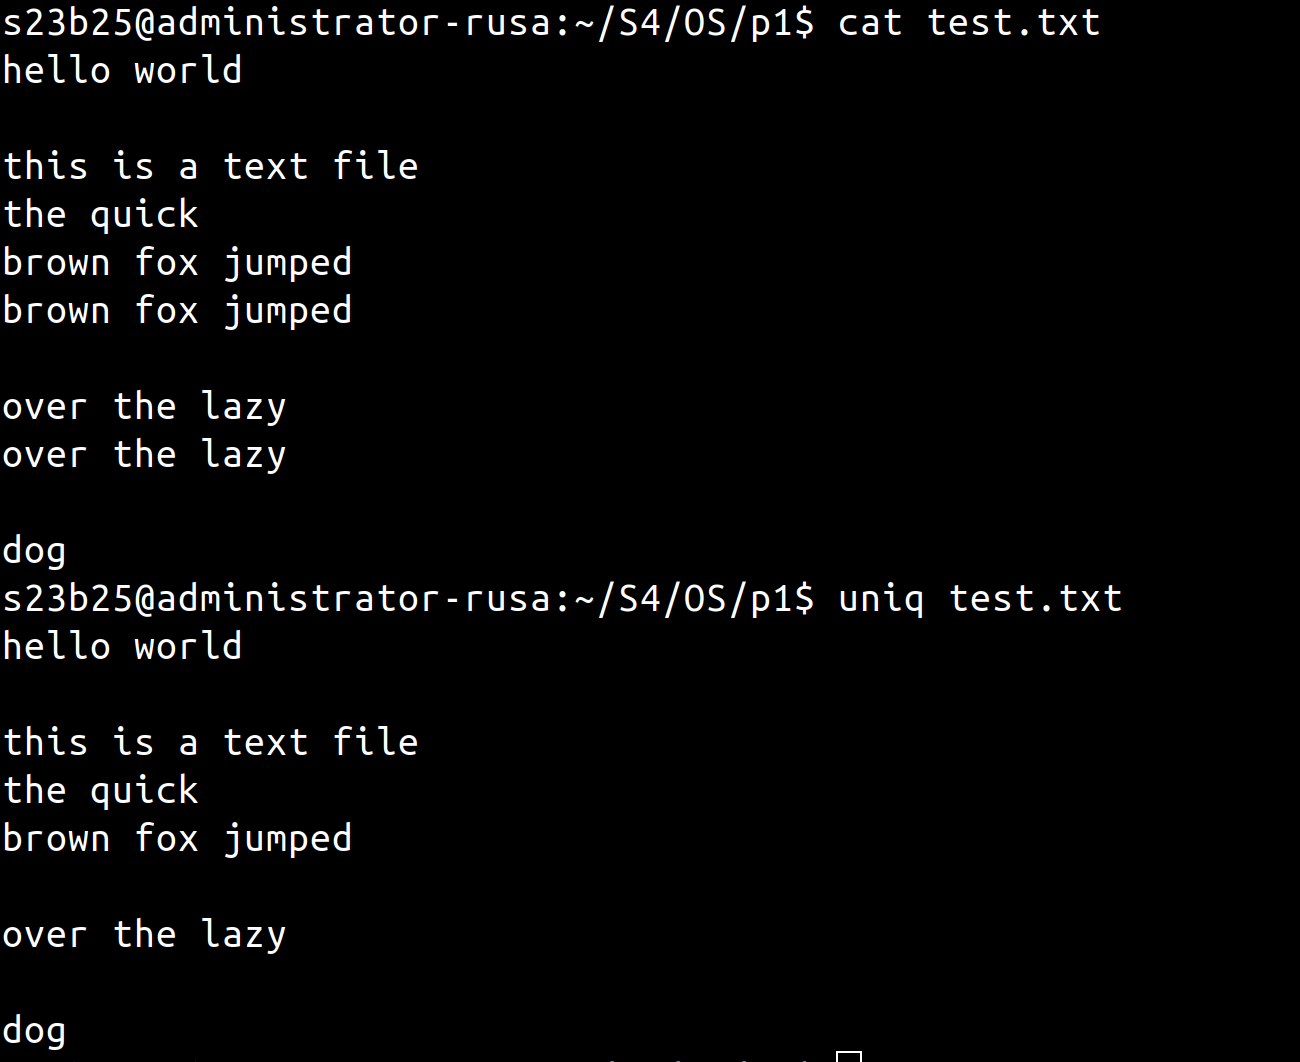
\includegraphics[width=\linewidth]{assets/uniq-1.png}
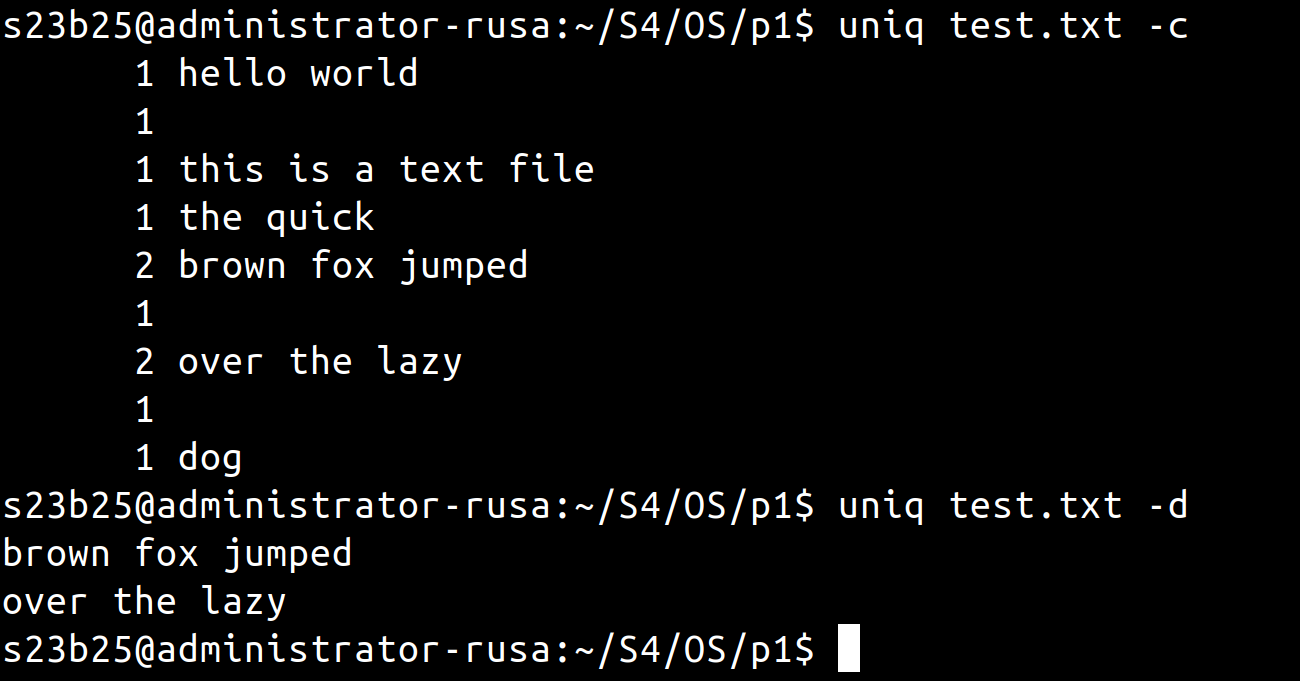
\includegraphics[width=\linewidth]{assets/uniq-2.png}
\end{minipage}
} %output screenshot name
\end{figure}
\subsection{Command 38: du} 
\textbf{Purpose}
\begin{flushleft}
 display disk usage statistics
\end{flushleft}
\textbf{Usage}
\begin{verbatim}
du
du -sh .
du -b
\end{verbatim}
\textbf{Sample i/p and o/p}
\begin{figure}[H] 
\fbox{
\begin{minipage}{350px} 
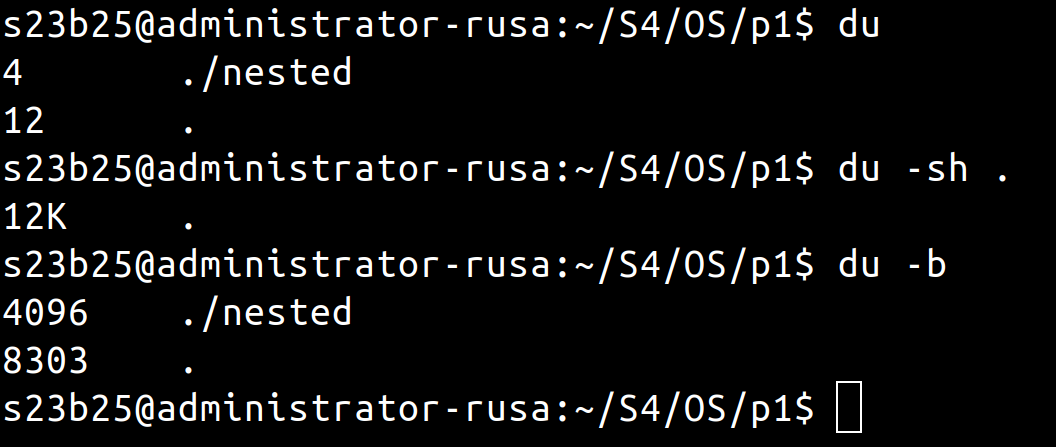
\includegraphics[width=\linewidth]{assets/du-1.png}
\end{minipage}
} %output screenshot name
\end{figure}
\subsection{Command 39: df} 
\textbf{Purpose}
\begin{flushleft}
 display free disk space
\end{flushleft}
\textbf{Usage}
\begin{verbatim}
df
df -h
\end{verbatim}
\textbf{Sample i/p and o/p}
\begin{figure}[H] 
\fbox{
\begin{minipage}{350px} 
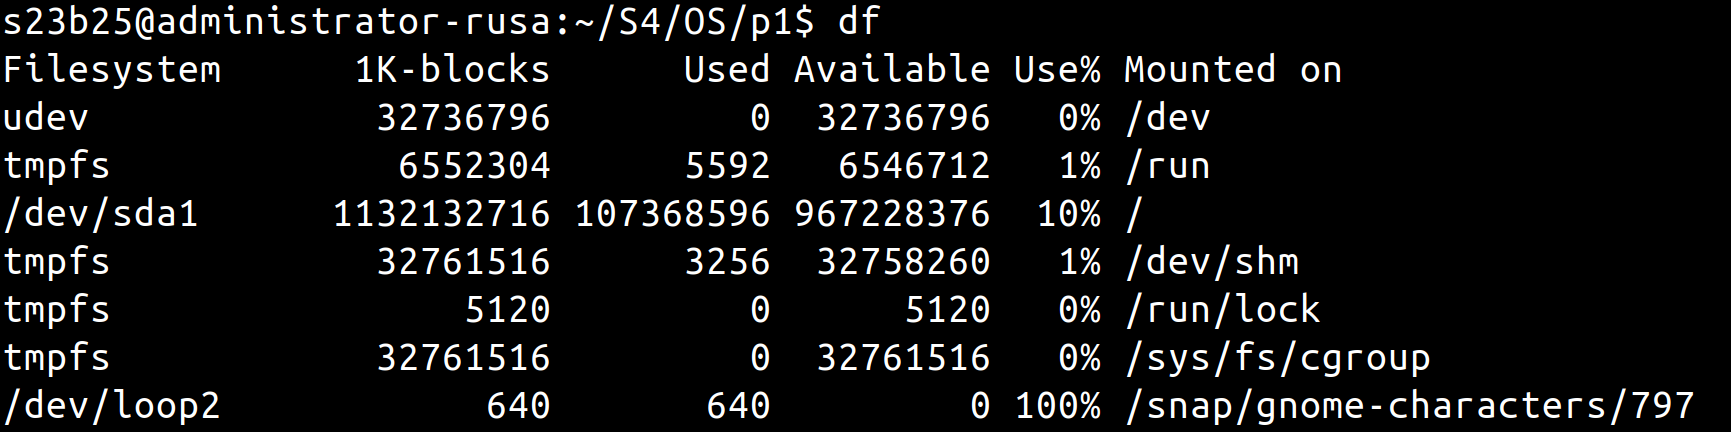
\includegraphics[width=\linewidth]{assets/df-1.png}
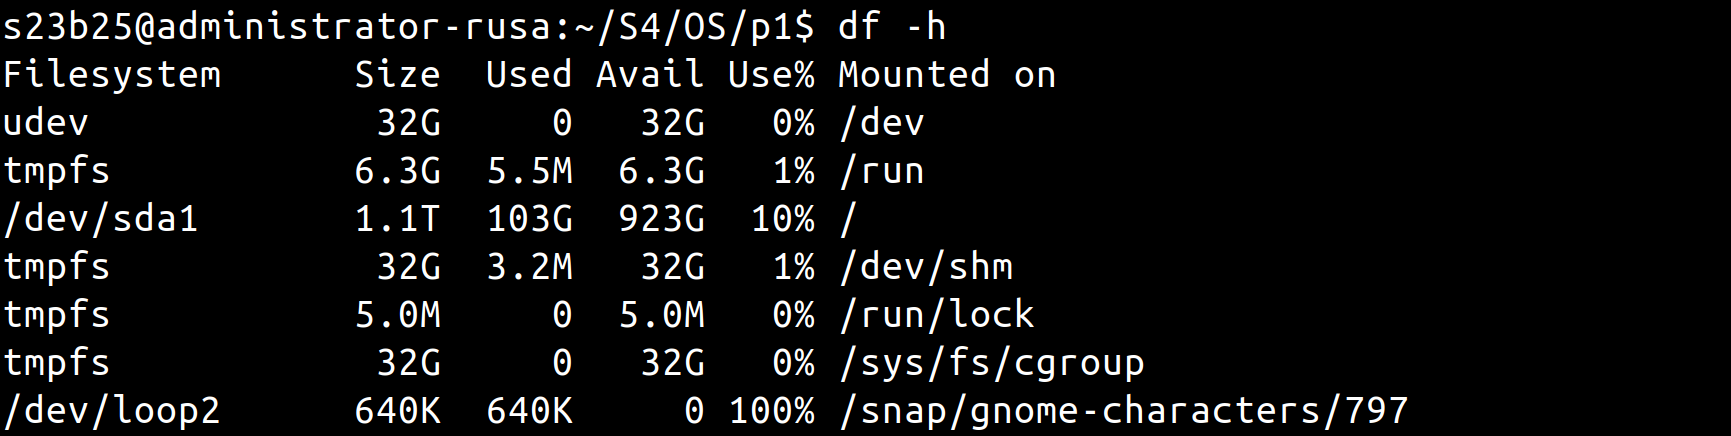
\includegraphics[width=\linewidth]{assets/df-2.png}
\end{minipage}
} %output screenshot name
\end{figure}
\subsection{Command 40: man} 
\textbf{Purpose}
\begin{flushleft}
 display online manual documentation pages
\end{flushleft}
\textbf{Usage}
\begin{verbatim}
man man
man -k debugger
man -f smail
\end{verbatim}
\textbf{Sample i/p and o/p}
\begin{figure}[H] 
\fbox{
\begin{minipage}{350px} 
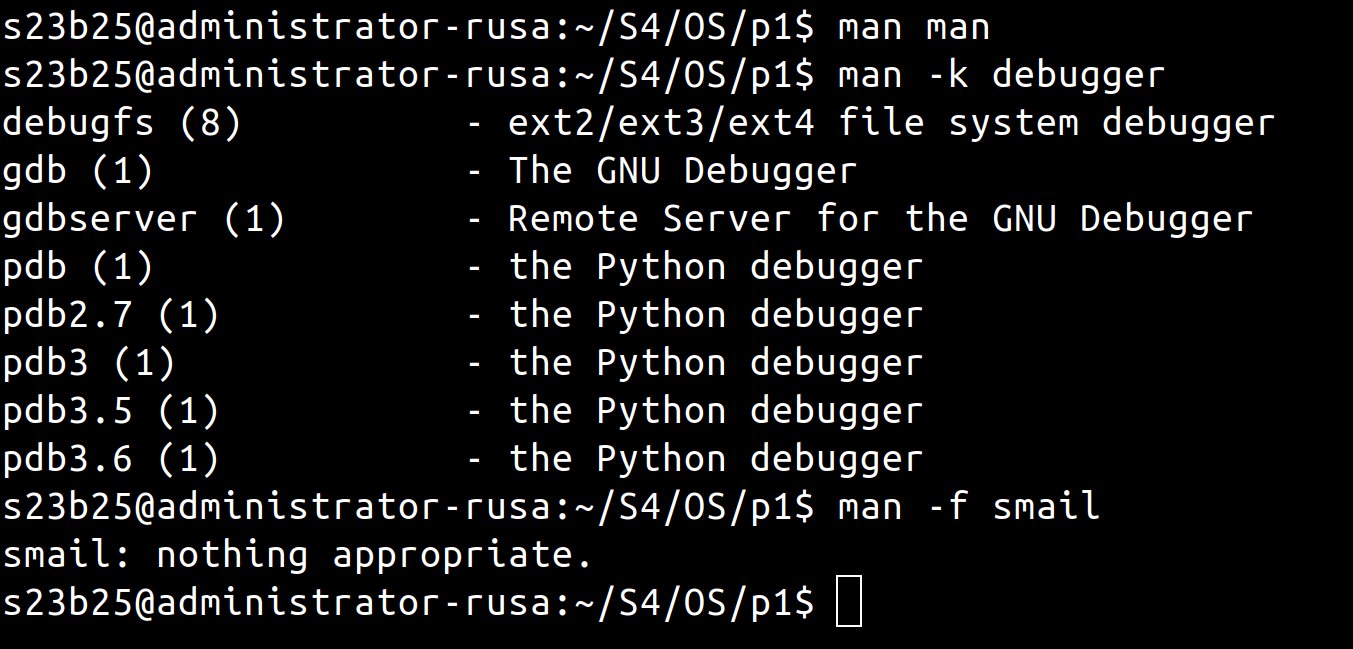
\includegraphics[width=\linewidth]{assets/man-1.png}
\end{minipage}
} %output screenshot name
\end{figure}
\subsection{Command 41: help} 
\textbf{Purpose}
\begin{flushleft}
display information about builtin commands
\end{flushleft}
\textbf{Usage}
\begin{verbatim}
help
\end{verbatim}
\textbf{Sample i/p and o/p}
\begin{figure}[H] 
\fbox{
\begin{minipage}{350px} 
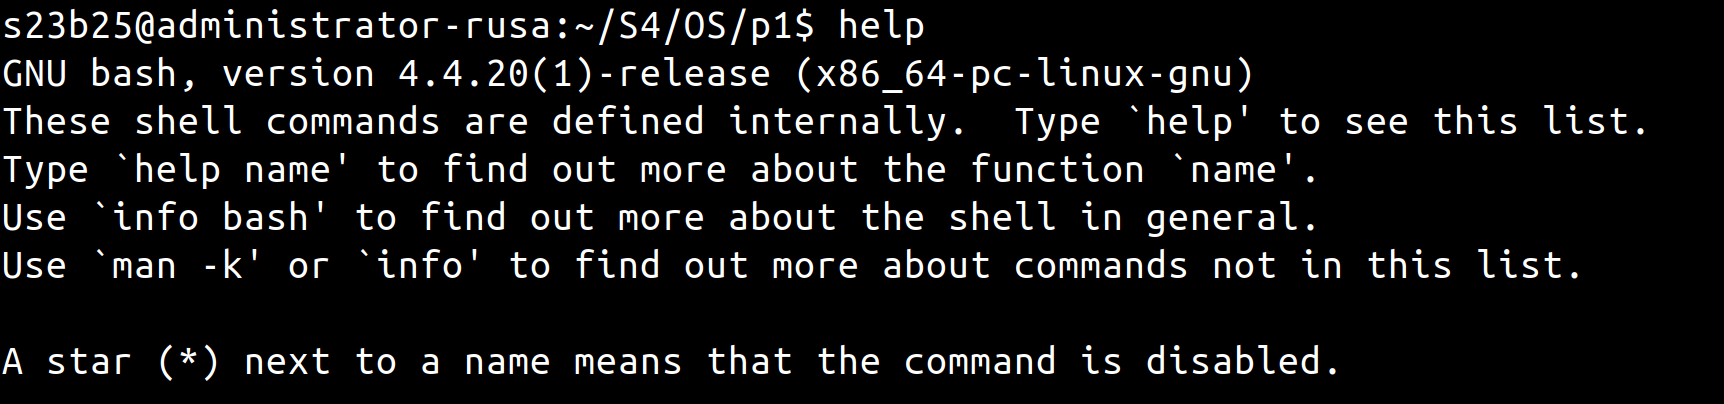
\includegraphics[width=\linewidth]{assets/help-1.png}
\end{minipage}
} %output screenshot name
\end{figure}
\subsection{Command 42: pr} 
\textbf{Purpose}
\begin{flushleft}
 print files
\end{flushleft}
\textbf{Usage}
\begin{verbatim}
pr test.txt
pr test.txt -d
pr test.txt -n
\end{verbatim}
\textbf{Sample i/p and o/p}
\begin{figure}[H] 
\fbox{
\begin{minipage}{350px} 
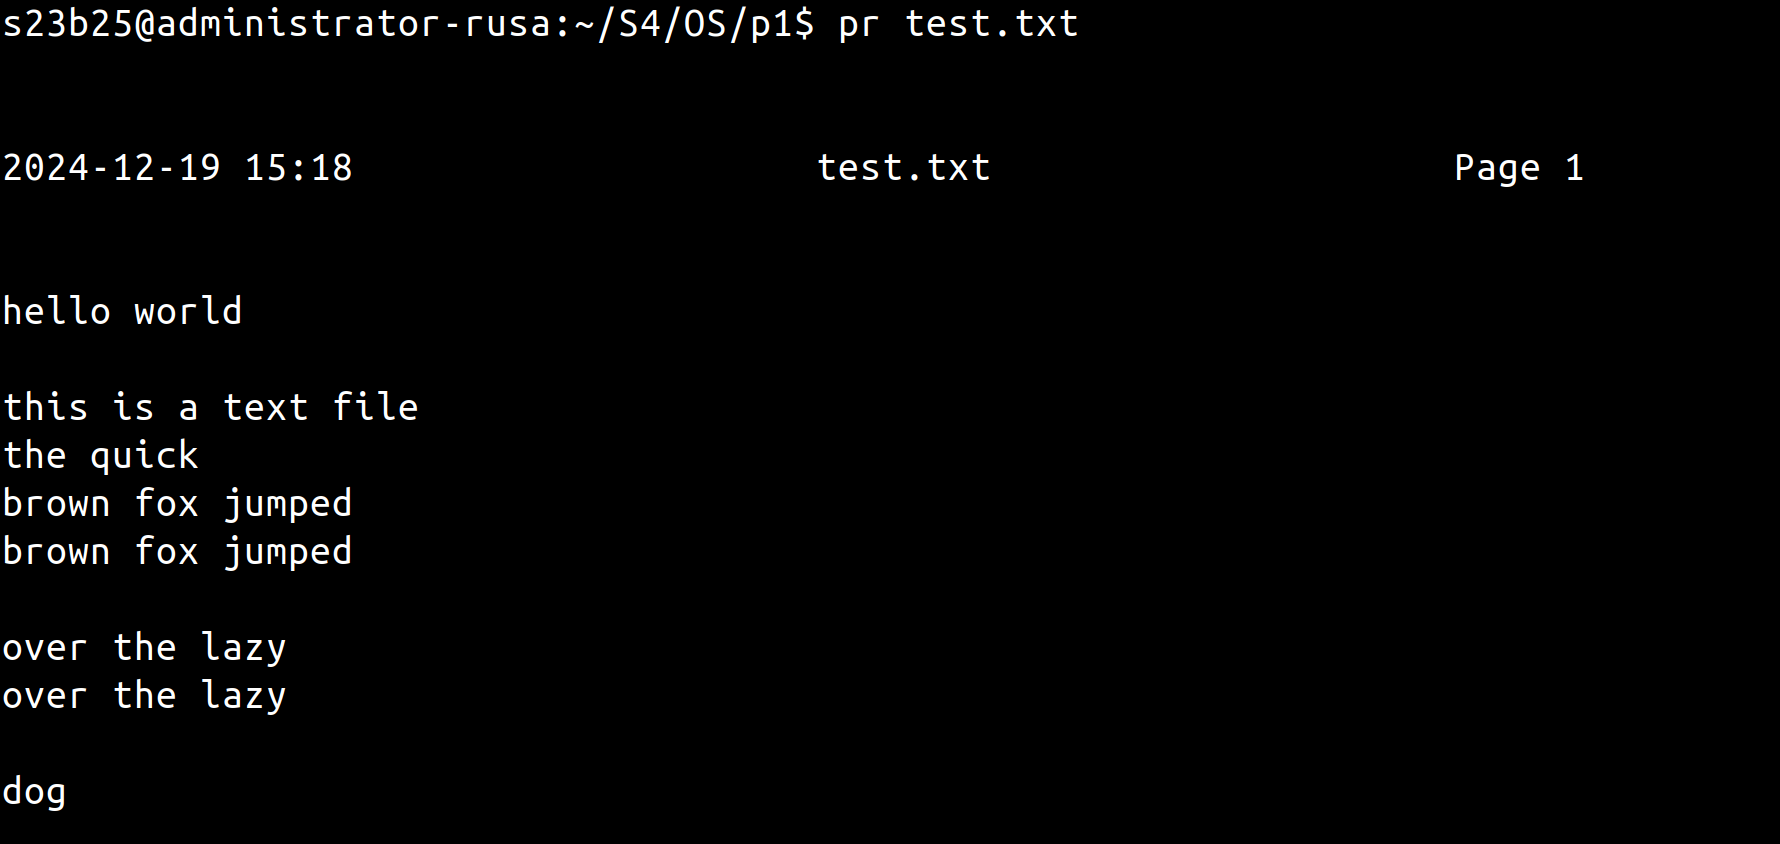
\includegraphics[width=\linewidth]{assets/pr-1.png}
\includegraphics[width=\linewidth]{assets/pr-2.png}
\includegraphics[width=\linewidth]{assets/pr-3.png}
\end{minipage}
} %output screenshot name
\end{figure}
\subsection{Command 43: tr} 
\textbf{Purpose}
\begin{flushleft}
 translate characters
\end{flushleft}
\textbf{Usage}
\begin{verbatim}
tr abc xyz
tr -c abc xyz
\end{verbatim}
\textbf{Sample i/p and o/p}
\begin{figure}[H] 
\fbox{
\begin{minipage}{350px} 
\includegraphics[width=\linewidth]{assets/tr-1.png}
\end{minipage}
} %output screenshot name
\end{figure}
\subsection{Command 44: diff} 
\textbf{Purpose}
\begin{flushleft}
 differential file and directory comparator
\end{flushleft}
\textbf{Usage}
\begin{verbatim}
diff test.txt testMod.txt
\end{verbatim}
\textbf{Sample i/p and o/p}
\begin{figure}[H] 
\fbox{
\begin{minipage}{350px} 
\includegraphics[width=\linewidth]{assets/diff-1.png}
\end{minipage}
} %output screenshot name
\end{figure}
\subsection{Command 45: wc} 
\textbf{Purpose}
\begin{flushleft}
 word, line, character, and byte count
\end{flushleft}
\textbf{Usage}
\begin{verbatim}
wc test.txt
wc test.txt -c
wc test.txt -l
wc test.txt -L
\end{verbatim}
\textbf{Sample i/p and o/p}
\begin{figure}[H] 
\fbox{
\begin{minipage}{350px} 
\includegraphics[width=\linewidth]{assets/wc-1.png}
\end{minipage}
} %output screenshot name
\end{figure}
\subsection{Command 46: bc} 
\textbf{Purpose}
\begin{flushleft}
       bc - arbitrary-precision decimal arithmetic language and calculator
\end{flushleft}
\textbf{Usage}
\begin{verbatim}
bc
\end{verbatim}
\textbf{Sample i/p and o/p}
\begin{figure}[H] 
\fbox{
\begin{minipage}{350px} 
\includegraphics[width=\linewidth]{assets/bc-1.png}
\end{minipage}
} %output screenshot name
\end{figure}
\subsection{Command 47: gzip} 
\textbf{Purpose}
\begin{flushleft}
 compression/decompression tool using Lempel-Ziv
\end{flushleft}
\textbf{Usage}
\begin{verbatim}
gzip test.txt
\end{verbatim}
\textbf{Sample i/p and o/p}
\begin{figure}[H] 
\fbox{
\begin{minipage}{350px} 
\includegraphics[width=\linewidth]{assets/gzip-1.png}
\end{minipage}
} %output screenshot name
\end{figure}
\subsection{Command 48: history} 
\textbf{Purpose}
\begin{flushleft}
     bbuuiillttiinn, !!, %%, .., ::, @@, [[, {{, }}, aalliiaass, aalllloocc, bbgg, bbiinndd, bbiinnddkkeeyy, bbrreeaakk,
\end{flushleft}
\textbf{Usage}
\begin{verbatim}
history
\end{verbatim}
\textbf{Sample i/p and o/p}
\begin{figure}[H] 
\fbox{
\begin{minipage}{350px} 
\includegraphics[width=\linewidth]{assets/history-1.png}
\end{minipage}
} %output screenshot name
\end{figure}
\subsection{Command 49: groups} 
\textbf{Purpose}
\begin{flushleft}
 show group memberships
\end{flushleft}
\textbf{Usage}
\begin{verbatim}
groups
\end{verbatim}
\textbf{Sample i/p and o/p}
\begin{figure}[H] 
\fbox{
\begin{minipage}{350px} 
\includegraphics[width=\linewidth]{assets/groups-1.png}
\end{minipage}
} %output screenshot name
\end{figure}
\subsection{Command 50: cut} 
\textbf{Purpose}
\begin{flushleft}
 cut out selected portions of each line of a file
\end{flushleft}
\textbf{Usage}
\begin{verbatim}
cut --characters=3 testMod.txt
\end{verbatim}
\textbf{Sample i/p and o/p}
\begin{figure}[H] 
\fbox{
\begin{minipage}{350px} 
\includegraphics[width=\linewidth]{assets/cut-1.png}
\end{minipage}
} %output screenshot name
\end{figure}
\end{document}
